% =====================================================================
% Mirante dos Dados — Working Paper #7 (v2.0)
% A Geografia Municipal do Bolsa Família: Heterogeneidade Intra-UF Real,
% Concentração Espacial e Diagnóstico de 5.570 Pontos de Decisão (2018–2025)
%
% Autor: Leonardo Chalhoub
% Versão: 2.0 — Abril de 2026 (rewrite from scratch — substitui v1.0 que
%        usava fallback UF→município com heterogeneidade intra-UF artificial =0).
%        Agora com dados REAIS via agregação direta de bronze.pbf_pagamentos
%        (2,53 bilhões de linhas, CGU Portal da Transparência) por município
%        × ano, joinado com geobr (IPEA) + IBGE/SIDRA pop municipal.
% Compilação: pdflatex articles/bolsa-familia-municipios.tex (2x)
% =====================================================================

\documentclass[12pt,a4paper,oneside]{article}

\usepackage[T1]{fontenc}
\usepackage[utf8]{inputenc}
\usepackage[brazilian]{babel}
\usepackage{newtxtext}
\usepackage{newtxmath}
\usepackage[section]{placeins}
\usepackage[a4paper,top=3cm,bottom=2cm,left=3cm,right=2cm]{geometry}
\usepackage{setspace}
\usepackage{indentfirst}
\usepackage{titlesec}
\usepackage{caption}
\usepackage{booktabs}
\usepackage{array}
\usepackage{multirow}
\usepackage{graphicx}
\usepackage[colorlinks=true,urlcolor=blue!60!black,linkcolor=black,citecolor=black,breaklinks=true]{hyperref}
\usepackage{url}
\usepackage{xurl}
\Urlmuskip=0mu plus 1mu\relax
\usepackage{float}
\usepackage{tcolorbox}

\graphicspath{{figures-pbf-municipios-v2/}}

\onehalfspacing
\setlength{\parindent}{1.25cm}
\setlength{\parskip}{0pt}

\titleformat{\section}{\normalfont\bfseries\large\uppercase}{\thesection}{0.6em}{}
\titleformat{\subsection}{\normalfont\bfseries\normalsize}{\thesubsection}{0.6em}{}
\titlespacing*{\section}{0pt}{18pt}{8pt}
\titlespacing*{\subsection}{0pt}{12pt}{6pt}

\captionsetup[table]{labelfont=bf,name=Tabela,labelsep=endash,position=above,justification=centering,font=small}
\captionsetup[figure]{labelfont=bf,name=Figura,labelsep=endash,position=below,justification=centering,font=small}
\captionsetup{skip=6pt}

\newcommand{\rs}{R\$\,}
\newcommand{\xurl}[2]{\url{#1}\,(acesso: #2)}

% Stamp de compilação injetado pelo CI (deploy-pages.yml).
% Para builds locais, este arquivo default é usado — basta um pdflatex direto
% e a capa exibe "(dev local)". Em CI, este arquivo é sobrescrito antes da
% compilação com timestamp BRT + SHA do commit que disparou o deploy.
\newcommand{\COMPILESTAMP}{compila\c{c}\~ao local}
\newcommand{\COMPILESHA}{dev}


\begin{document}

% ---------- CAPA -------------------------------------------------------
\begin{titlepage}
  \begin{center}
    \vspace*{1.5cm}
    {\small\textsc{Mirante dos Dados \quad\textbar\quad Working Paper n. 7}}\\
    {\small Versão 2.0 \textemdash{} Abril de 2026}\\[2pt]
    {\footnotesize Compilada em \COMPILESTAMP\ \textbullet\ \texttt{\COMPILESHA}}

    \vfill

    {\LARGE\bfseries
     A GEOGRAFIA MUNICIPAL DO BOLSA FAMÍLIA:

     HETEROGENEIDADE INTRA-UF REAL,
     CONCENTRAÇÃO ESPACIAL E
     DIAGNÓSTICO DE
     5.570 PONTOS DE DECISÃO

     (2018\textendash 2025)}

    \vspace{1cm}
    {\large\itshape
     The municipal geography of Bolsa Família: real intra-state heterogeneity,
     spatial concentration, and a diagnostic of 5{,}570 decision points
     (2018\textendash 2025)}

    \vfill

    {\large\textbf{Leonardo Chalhoub}}\\[4pt]
    {\small Pesquisador independente \textemdash{} engenharia de dados,
     análise espacial, decomposição Theil within/between,
     pipeline reproduzível em escala de Big Data.}\\[2pt]
    {\small\href{mailto:leonardochalhoub@gmail.com}{leonardochalhoub@gmail.com}}\\
    {\small\href{https://github.com/leonardochalhoub/mirante-dos-dados-br}{github.com/leonardochalhoub/mirante-dos-dados-br}}

    \vfill

    {\small Brasil \\ Abril de 2026}\\[6pt]
    {\footnotesize\textit{Citar como:}\\[2pt]
     Chalhoub, L. (2026). \textit{A geografia municipal do Bolsa Família:
     heterogeneidade intra-UF real, concentração espacial e diagnóstico
     de 5.570 pontos de decisão (2018\textendash 2025).}
     Mirante dos Dados — Working Paper n.\,7, v.\,2.0.\\
     Disponível em: \url{https://leonardochalhoub.github.io/mirante-dos-dados-br/}.
     Acesso em: \COMPILESTAMP.}
  \end{center}
\end{titlepage}

% ---------- RESUMO -----------------------------------------------------
\section*{Resumo}
\addcontentsline{toc}{section}{Resumo}

Este Working Paper analisa o programa Bolsa Família\,/\,Auxílio Brasil\,/\,Novo
Bolsa Família (PBF\,/\,AB\,/\,NBF) em granularidade \textbf{municipal} para os
\textbf{5.570 municípios brasileiros}, no período 2018\textendash 2025. Substitui
o painel UF\,$\times$\,Ano do Working Paper n.\,2 do Mirante dos Dados
(Chalhoub, 2026)\,---\,que documentou três regimes institucionais e identificou
causalmente o salto da MP 1.061/2021\,---\,por um painel
Município\,$\times$\,Ano com cobertura completa. A motivação central é que a
\textbf{análise estadual oculta, por construção, a desigualdade intra-UF}: a
hipótese de homogeneidade dentro do estado é falsa pela própria mecânica da
focalização do programa, que opera no nível individual via Cadastro Único e
não por agregação geográfica.

A construção de dados parte da agregação direta de
\textbf{2{,}53 bilhões} de linhas de pagamentos individuais publicados pelo
Portal da Transparência da CGU (Lei 12.527/2011) sobre o cluster
\texttt{mirante\_prd.bronze.pbf\_pagamentos}, joinada com a tabela canônica
do IPEA \texttt{geobr.read\_municipality} (5.570 polígonos com código IBGE
de 7 dígitos) e estimativas populacionais municipais do IBGE/SIDRA Tabela
6579. O pipeline é reproduzível em sua totalidade no repositório
\texttt{mirante-dos-dados-br}; o lookup IBGE\,$\leftrightarrow$\,CGU resolve
\textbf{100\,\% dos 5.570 municípios} (5.545 por normalização Unicode +
\textit{strip} de acentos; 25 por mapeamento manual UF-aware das divergências
ortográficas históricas catalogadas, e.g.\ \textit{Brazópolis} vs
\textit{BRASOPOLIS}, \textit{Itapajé} vs \textit{ITAPAGE}, \textit{Paraty}
vs \textit{PARATI}).

Os achados centrais quantificam pela primeira vez, em escala municipal e
com dados oficiais, três fenômenos: (i) a desigualdade intra-UF
\textbf{representa 33{,}6\,\% da variância total} do PBF per capita
(decomposição de Theil L) — o WP\,n.\,2 não conseguia observar nada deste
componente por construção do painel; (ii) os \textbf{top 100 municípios
concentram 32{,}4\,\%} dos R\$\,156{,}4 bilhões de transferência total em
2025, indicando \textit{spatial sorting} compatível com a focalização
declarada; (iii) o \textit{range} de PBF per capita
\textbf{varia de \rs 13/hab a \rs 3.536/hab} (razão 271$\times$), com Serrano
do Maranhão\,---\,MA no topo (\rs 3.536/hab, 49{,}9\,\% da população
beneficiária) e Pomerode\,---\,SC na base (\rs 13/hab, 0{,}26\,\% da população
beneficiária); a diferença é compatível com a divisão histórica entre
sertão nordestino e colônias alemãs catarinenses.

Quinze figuras documentam a distribuição\,---\,5 mapas coropléticos em paletas
distintas (\textit{magma\_r, YlOrRd, cividis\_r, Greys, viridis\_r}; todas
\textit{colorblind-safe}) e 10 gráficos de histograma, Lorenz, top/bottom,
agregação regional, decomposição Theil, dispersão e concentração Pareto. A
limitação central é a ausência de identificação causal específica neste
WP\,---\,a contribuição é \textit{descriptive deepening} sobre o painel UF do
WP\,n.\,2, não substituição. A agenda imediata é replicar os desenhos DiD
sobre MP 1.061/2021 do WP\,n.\,2 com k\,=\,5.570 \textit{clusters}
municipais, usando Conley HAC com distâncias geodésicas reais.

\smallskip
\noindent\textbf{Palavras-chave}: Bolsa Família; análise espacial; município;
heterogeneidade intra-estadual; decomposição de Theil; geobr; choropleth;
\textit{Big Data} público brasileiro; Portal da Transparência;
reprodutibilidade.

% ---------- ABSTRACT --------------------------------------------------
\section*{Abstract}
\addcontentsline{toc}{section}{Abstract}

This Working Paper analyses Brazil's Bolsa Família\,/\,Auxílio
Brasil\,/\,Novo Bolsa Família program (PBF/AB/NBF) at a \textbf{municipal}
granularity covering all \textbf{5{,}570 Brazilian municipalities} from
2018 to 2025. It complements Working Paper n.\,2 (Chalhoub, 2026) by
replacing the state\,$\times$\,year panel with a municipality\,$\times$\,year
panel of full coverage. The motivation is that state-level analysis
structurally hides intra-state heterogeneity: the assumption of within-state
homogeneity is false by program design (means-tested at the individual level
through the Cadastro Único, not geographically aggregated).

Data construction starts from direct aggregation of \textbf{2.53 billion}
individual payment rows published by Brazil's Federal Comptroller (CGU)
under the Transparency Portal (Law 12,527/2011) over the
\texttt{mirante\_prd.bronze.pbf\_pagamentos} cluster, joined with the IPEA
canonical table \texttt{geobr.read\_municipality} (5{,}570 polygons with
7-digit IBGE codes) and IBGE/SIDRA Table 6579 municipal population
estimates. IBGE\,$\leftrightarrow$\,CGU lookup resolves
\textbf{100\,\% of the 5{,}570 municipalities}.

Central findings: (i) intra-state heterogeneity \textbf{accounts for
33.6\,\%} of total per-capita PBF variance (Theil L decomposition) — invisible
in the state-level panel; (ii) the \textbf{top 100 municipalities receive
32.4\,\%} of the R\$\,156.4 billion total transfer in 2025; (iii) per-capita
PBF \textbf{ranges from R\$\,13 to R\$\,3{,}536} (271$\times$ ratio), with
Serrano do Maranhão (MA) at the top and Pomerode (SC) at the bottom.

Five \textit{colorblind-safe} maps and ten supporting charts (histogram,
Lorenz, top/bottom rankings, regional aggregates, Theil decomposition,
density-PBF scatter, Pareto concentration) document the panel. The main
limitation is the absence of \textit{ad-hoc} causal identification — the
contribution is \textit{descriptive deepening} of WP n.\,2, not replacement.

\smallskip
\noindent\textbf{Keywords}: Bolsa Família; spatial analysis; municipality;
intra-state heterogeneity; Theil decomposition; geobr; choropleth.

\clearpage

% =====================================================================
\section{Introdução}\label{sec:intro}

O Programa Bolsa Família, criado pela Lei n.\,10.836, de 9 de janeiro de
2004 (Brasil, 2004), foi por duas décadas a maior política brasileira de
transferência condicional de renda. O Working Paper n.\,2 do Mirante dos
Dados (Chalhoub, 2026)\,---\,doravante \textit{WP\,2}\,---\,documentou os
três regimes pelos quais o programa atravessou: o PBF clássico
(2003\textendash 2021), o Auxílio Brasil instituído pela Medida Provisória
1.061/2021 e convertida na Lei 14.284/2021, e o Novo Bolsa Família
estabelecido pela Lei 14.601/2023. O \textit{WP\,2} produziu identificação
causal sobre o salto da MP 1.061/2021 via diferença-em-diferenças (DiD)
\textit{two-way fixed effects} clusterizado por UF, com \textit{wild-cluster
bootstrap} (Cameron, Gelbach \& Miller, 2008) para mitigar o problema de
poucos \textit{clusters} (N\,=\,27).

Este Working Paper\,---\,doravante \textit{WP\,7}\,---\,parte de uma observação
simples mas materialmente importante: \textbf{o painel UF\,$\times$\,ano do WP\,2
não consegue observar a desigualdade dentro do estado}. A hipótese de
homogeneidade dentro da UF é \textit{falsa por construção do programa}: o
PBF é \textit{means-tested} no nível individual\,/\,familiar via Cadastro
Único Federal\,---\,um cidadão de Pomerode\,---\,SC e um de Serrano do
Maranhão\,---\,MA são avaliados com o mesmo critério de renda nominal,
independentemente da UF que habitam. A focalização emergente é resultado
de \textit{taxas regionais de pobreza}, não de agregação estadual. Logo, a
agregação ao nível UF mistura pobres do litoral nordestino com pobres do
sertão; mistura ricos da capital paulista com pobres do Vale do Ribeira;
mistura colônias alemãs do Sul com periferias urbanas da mesma região. O
preço dessa mistura é a perda informacional sobre \textit{onde} de fato
chegam os \rs 156{,}4 bilhões anuais do programa (R\$ nominais 2025; vide
Seção\,\ref{sec:eda}).

A pergunta central de pesquisa do \textit{WP\,7} é: \textit{quanto da
desigualdade total do PBF per capita é entre estados (\textit{between}) e
quanto é dentro deles (\textit{within})?} Uma resposta principial requer
três insumos que o \textit{WP\,2} não tinha: (i) painel municipal completo,
i.e.\ não-amostral, dos 5.570 municípios brasileiros; (ii) decomposição
formal\,---\,Theil L\,---\,da variância total nas componentes within e between;
(iii) cobertura temporal suficiente para distinguir composição transversal
(corte 2025) de dinâmica longitudinal (variação 2018\,$\rightarrow$\,2025
deflacionada).

A construção de dados\,---\,ver Seção\,\ref{sec:metodo}\,---\,parte dos
\textbf{2{,}53 bilhões de linhas} de pagamentos individuais publicados pela
CGU no Portal da Transparência (Lei n.\,12.527, de 18 de novembro de 2011),
em arquivos CSV mensais agregados em uma tabela bronze
\texttt{mirante\_prd.bronze.pbf\_pagamentos}. Esses dados não são tratáveis
em planilhas eletrônicas\,---\,um único mês ultrapassa o limite de
1.048.576 linhas do Excel; processamento via \textit{Big Data} stack
(Spark\,/\,Delta\,/\,SQL warehouse) é, na prática, condição necessária para
a operação. A agregação a Município\,$\times$\,Ano produz 5.571
\textit{groups} (1 ``órfão'' do CGU, ``Boa Esperança do Norte\,---\,MT'',
sem código IBGE oficial, deve ser tratado em pipeline futura) que
joinamos com o pacote \texttt{geobr} (Pereira \& Gonçalves, 2022; \textit{port}
em Python por \texttt{ipeaGIT/geobr}) que retorna 5.570 municípios IBGE
oficiais com geometria simplificada.

A escolha do \texttt{geobr} sobre alternativas (CSV de referência manual,
IBGE/MalhaDigital API com 5.570 chamadas, snapshot de \textit{shapefile}
desatualizado) é pragmática: é o pacote canônico mantido pelo Instituto de
Pesquisa Econômica Aplicada (IPEA), com paridade direta entre R e Python,
fornecendo simultaneamente metadata (\texttt{code\_muni},
\texttt{name\_muni}, \texttt{abbrev\_state}) e geometria de plotagem
\textit{out-of-the-box}.

A estrutura adotada\,---\,15 figuras (5 mapas + 10 gráficos), 4 tabelas
diagnósticas\,---\,combina visualização cartográfica com inferência
quantitativa formal. A contribuição do \textit{WP\,7} é \textit{descriptive
deepening} sobre o \textit{WP\,2}, não substituição. Identificação causal
específica fica como agenda imediata: replicar os desenhos DiD sobre MP
1.061/2021 com k\,=\,5.570 \textit{clusters} municipais, eliminando o problema
de poucos \textit{clusters} que motivou o \textit{wild-cluster bootstrap} no
WP\,2. Conley HAC (Conley, 1999) com distâncias geodésicas reais
(\textit{haversine} entre centroides via \texttt{geobr}, \textit{bandwidth}
\textit{sensitivity} 50\,---\,1.600\,km) será implementado em iteração
subsequente.

% =====================================================================
\section{Histórico Institucional}\label{sec:historico}

Esta seção é deliberadamente \textit{condensada}. O leitor que busca
detalhes legais e cronologia institucional plena deve consultar a Seção\,2
do \textit{WP\,2} (Chalhoub, 2026). Aqui apresentamos apenas o estritamente
necessário para que o leitor compreenda a interpretação dos saltos
de 2021 e 2023 visíveis nos mapas e na dinâmica 2018\,$\rightarrow$\,2025.

\subsection{Bolsa Família (Lei 10.836/2004 — out./2003 a out./2021)}
Programa criado pelo Decreto n.\,5.209/2004 unificando os pré-existentes
Bolsa Escola, Bolsa Alimentação, Auxílio Gás e Cartão Alimentação. O valor
mínimo era de \rs 89/mês por família em 2018, com adicionais por gestante,
nutriz, criança, adolescente e responsável (Brasil, 2004; Decreto
6.917/2009).

\subsection{Auxílio Brasil (MP 1.061/2021 → Lei 14.284/2021)}
Em 9/8/2021 o governo federal substituiu o PBF pelo Auxílio Brasil,
elevando o piso para \rs 400/mês e ampliando a cobertura. A medida
provisória 1.061/2021 foi convertida na Lei 14.284 de 29/12/2021. O
benefício foi posteriormente elevado para \rs 600/mês via PEC dos
Combustíveis (Emenda Constitucional 123/2022, em 14/7/2022,
às vésperas da campanha eleitoral). O \textit{WP\,2} identificou o salto
da MP 1.061/2021 como o maior choque institucional do programa em duas
décadas (DiD\,$\beta$\,$\approx$\,+\rs 95/hab, p\,$<$\,0{,}05).

\subsection{Novo Bolsa Família (Lei 14.601/2023)}
Em 28/3/2023, o NBF retomou o nome \textit{Bolsa Família} mas com
estrutura redesenhada: piso de \rs 600/família, adicional de \rs 150 por
criança $<$\,7 anos e \rs 50 por gestante, nutriz e jovem 7\,---\,18 anos
(Brasil, 2023). O número de famílias beneficiárias estabilizou em
$\sim$20{,}5\,milhões em 2024\,---\,2025.

\subsection{Marcos institucionais visíveis nos dados}
O \textit{WP\,7} não reidentifica esses marcos\,---\,o \textit{WP\,2} já o fez
no nível UF. O leitor deve interpretar o crescimento de 2018\,$\rightarrow$\,2025
visível no Mapa\,5 e na Figura\,14 como o efeito \textit{cumulativo} desses três
regimes sobre cada município, não atribuível a um único choque.

% =====================================================================
\section{Metodologia}\label{sec:metodo}

\subsection{Fontes de dados primárias}
\begin{itemize}\itemsep4pt
\item \textbf{CGU\,/\,Portal da Transparência\,---\,Bolsa Família,
  Auxílio Brasil, Novo Bolsa Família.} Microdados mensais de pagamentos
  individuais (\textit{NIS, nome, CPF mascarado, valor, mês de
  competência, mês de referência, código SIAFI do município, nome do
  município, UF}). Cobertura jan/2013 a abr/2026. Total bronze:
  2{,}53\,bilhões de linhas.
  \xurl{https://portaldatransparencia.gov.br/download-de-dados/bolsa-familia-pagamentos}{27\,abr.\,2026, 22h\,BRT}.
\item \textbf{IBGE\,/\,SIDRA Tabela 6579\,---\,Estimativas populacionais
  municipais.} Variável 9324, nível N6 (município). Cobertura 2013\,---\,2024
  (estimativas) + 2022 (Censo, via Tabela 4709). Para 2023 IBGE não
  publicou estimativa direta (\textit{gap} pós-Censo); silver interpola
  linearmente entre 2022 (Censo) e 2024 (Estimativa).
  \xurl{https://sidra.ibge.gov.br/tabela/6579}{27\,abr.\,2026, 21h\,BRT}.
\item \textbf{IBGE\,/\,SIDRA Tabela 1301\,---\,Áreas territoriais.} Variável
  632, nível N6, último período publicado.
  \xurl{https://sidra.ibge.gov.br/tabela/1301}{27\,abr.\,2026, 21h\,BRT}.
\item \textbf{IPEA \texttt{geobr} (Python port).} Pacote canônico mantido
  pelo IPEA com a malha digital municipal IBGE 2020 (5.570 polígonos),
  metadata (\texttt{code\_muni}, \texttt{name\_muni},
  \texttt{abbrev\_state}, \texttt{name\_state}, \texttt{name\_region}) e
  geometria simplificada para \textit{plotting}.
  \xurl{https://github.com/ipeaGIT/geobr}{27\,abr.\,2026, 22h\,BRT};
  \xurl{https://pypi.org/project/geobr/}{27\,abr.\,2026, 22h\,BRT}.
\item \textbf{BCB\,/\,SGS série 433 (IPCA mensal).} Deflator IPCA
  acumulado 2018\,$\rightarrow$\,2025: 41{,}5\,\% (Banco Central do Brasil,
  2026). Aplicado pelo silver \texttt{ipca\_deflators\_2021} no painel
  UF e replicado neste \textit{WP} para o painel municipal.
  \xurl{https://api.bcb.gov.br/dados/serie/bcdata.sgs.433/dados?formato=json}{27\,abr.\,2026, 21h\,BRT}.
\end{itemize}

\subsection{Pipeline de dados}\label{sec:metodo:pipeline}

A construção dos painéis municipais segue a arquitetura medallion
(\textit{bronze \(\to\) silver \(\to\) gold}) implementada em
\texttt{mirante\_prd} no Databricks, com \textit{Delta Lake} como formato
de tabela e \textit{Spark SQL} como motor de transformação. O código
completo está versionado em \texttt{pipelines/notebooks/} no repositório
\texttt{mirante-dos-dados-br}.

\paragraph{Bronze.} (a) \texttt{bronze.pbf\_pagamentos}: 2{,}53\,bi linhas,
\textit{string-only} por padrão da plataforma\,---\,nenhuma inferência de
tipo no bronze; \textit{cast} é obrigação do silver. (b)
\texttt{bronze.geobr\_municipios\_meta}: 5.570 munis com IBGE 7-dig +
nome + UF + região, \textit{ingest} via \texttt{\%pip install geobr}. (c)
\texttt{bronze.ibge\_municipios\_populacao\_raw}: payloads JSON da SIDRA
6579/N6 (2013\,---\,2024) com Censo 2022 da Tabela 4709/93 quando IBGE não
publicou estimativa. (d) \texttt{bronze.bcb\_ipca\_raw}: série 433 mensal
do BCB.

\paragraph{Silver.} (a) \texttt{silver.populacao\_municipio\_ano}: long
format (\texttt{Ano, cod\_municipio, municipio, uf, municipio\_uf,
populacao, populacao\_estimada, source}); 5.570\,$\times$\,12 anos =
$\sim$67k linhas; flag \texttt{populacao\_estimada} marca interpolação 2023.
(b) \texttt{silver.pbf\_total\_municipio\_mes}: 5.570\,$\times$\,$\sim$150
meses = $\sim$835k linhas, com \texttt{n\_distinct\_NIS}, \texttt{n\_ano},
\texttt{total\_municipio} (\textit{decimal} 38,2). \textit{Lookup} IBGE via
\texttt{(uf, normalize(nome\_municipio))} contra
\texttt{bronze.geobr\_municipios\_meta}, com mapeamento manual UF-aware
para 25 divergências ortográficas históricas. Após o fix, \textbf{100\,\% dos
5.570 municípios bate}.

\paragraph{Gold.} \texttt{gold.pbf\_municipios\_df}: painel
Município\,$\times$\,Ano final
(\texttt{Ano, cod\_municipio, municipio, uf, regiao, populacao,
n\_benef, valor\_nominal, valor\_2021, pbfPerBenef, pbfPerCapita}). $\sim$67k
linhas. Exporta para \texttt{gold/exports/gold\_pbf\_municipios\_df.json}
para consumo do front-end.

\subsection{Indicadores construídos}\label{sec:metodo:indicadores}

\begin{itemize}\itemsep3pt
\item \textbf{PBF per capita} = $\frac{\sum_{\text{ano}} \text{valor\_2021}}{\text{populacao}}$
  (\rs/hab/ano em moeda real 2021).
\item \textbf{PBF por beneficiário} = $\frac{\sum_{\text{ano}} \text{valor\_2021}}{n\_benef}$
  (\rs/família/ano em moeda real 2021).
\item \textbf{Cobertura} = $\frac{n\_benef}{\text{populacao}} \times 100$ (\,\% da
  população beneficiária; aproximação de famílias quando $\bar{f}$ fixo
  $\approx$\,3{,}1 pessoas).
\item \textbf{Densidade demográfica} = $\frac{\text{populacao}}{\text{area\_km}^2}$;
  \textit{area\_km}$^2$ computada de \texttt{geobr.geometry} em projeção
  EPSG:5880 (Brasil Polyconic), apropriada para análise nacional sem
  distorção de área (Snyder, 1987).
\item \textbf{Crescimento real} = $\left(\frac{\text{valor}_{2025} \cdot
  \delta_{2018}}{\text{valor}_{2018}} - 1\right)\times 100$ com $\delta_{2018}
  = \frac{1}{1{,}415}$ (deflator IPCA acumulado).
\end{itemize}

\subsection{Decomposição de Theil L (within / between UF)}\label{sec:metodo:theil}

A decomposição Theil L (Theil, 1972; Bourguignon, 1979) sobre a
distribuição municipal de PBF per capita é o instrumento formal que
quantifica a parcela da desigualdade total atribuível a (a)
\textit{between-UF}: diferenças entre médias estaduais; e
(b) \textit{within-UF}: dispersão dentro de cada estado. Definimos:
\[
L = \frac{1}{P} \sum_{i=1}^{N} p_i \cdot \log\!\left(\frac{\bar{x}}{x_i}\right)
\quad
L_w = \sum_{u\in\text{UF}} \frac{P_u}{P} \cdot L_u
\quad
L_b = L - L_w
\]
onde $x_i$ é PBF per capita do município $i$, $p_i$ é população, $P=\sum p_i$,
$\bar{x}$ é a média ponderada nacional e $L_u$ é o Theil dentro da UF $u$. A
propriedade aditiva ($L = L_w + L_b$) é garantida apenas em Theil
\textit{mean-log-deviation} (Theil L); Theil T tem decomposição diferente,
com base na média populacional (Cowell, 2000).

\subsection{Identificação geográfica e visualização}\label{sec:metodo:viz}

Cinco mapas coropléticos foram gerados a partir de \texttt{geobr.geometry}
(EPSG:4326 lat/lon) com \texttt{matplotlib} via \texttt{geopandas.plot}
(Jordahl et al., 2020; Hunter, 2007). Paletas escolhidas para
\textit{colorblind safety} usam o catálogo do
\texttt{matplotlib.colormaps} avaliado por
Wong (2011)\,---\,as variantes \texttt{magma\_r, YlOrRd, cividis\_r,
Greys, viridis\_r} são sequenciais, monotonicamente
percetíveis em deuteranopia, protanopia e tritanopia, e seguem o
sentido \textbf{claro\,=\,baixo $\rightarrow$ escuro\,=\,alto} requerido
para escalas de quantidade.

\subsection{Limitações declaradas}\label{sec:metodo:limites}

\begin{itemize}\itemsep3pt
\item Identificação causal \textbf{não} é apresentada neste WP. O DiD do
  WP\,2 sobre MP 1.061/2021 será replicado em iteração subsequente com
  k\,=\,5.570 \textit{clusters} municipais.
\item Crescimento real 2018$\to$2025 usa um único deflator nacional (IPCA
  acumulado). A inflação \textit{real} difere por UF/região; o Censo 2022
  detectou divergências entre IPCA e custo de vida regional. Esta
  aproximação é conservadora\,---\,corrigi-la favoreceria estados pobres
  do Norte/Nordeste.
\item População 2025 é aproximada por estimativa 2024 (IBGE não publica
  estimativa para o ano corrente). O erro é $\leq$\,1\,\% para a maioria
  dos municípios.
\item Cobertura é aproximada por $n_{\text{benef}}/p$. O programa paga
  por família, não por indivíduo. Aproximação por população é aceita na
  literatura (Soares, 2010; Higgins \& Pereira, 2014).
\end{itemize}

% =====================================================================
\section{Resultados Descritivos: o panorama nacional}\label{sec:eda}

\subsection{Totais agregados 2018 e 2025}

\begin{table}[H]
\centering\small
\caption{Totais nacionais agregados a partir de
\texttt{bronze.pbf\_pagamentos}}
\label{tab:totais}
\begin{tabular}{lrrr}
\toprule
\textbf{Indicador} & \textbf{2018} & \textbf{2025} & \textbf{$\Delta$ real} \\
\midrule
Beneficiários distintos por NIS (mi)        & 14{,}1 & 21{,}7 & +54\,\% \\
Valor total (R\$ bi nominal)                & 25{,}3 & 156{,}4 & --- \\
Valor total (R\$ bi 2018, deflacionado)     & 25{,}3 & 110{,}5 & +337\,\% \\
PBF per capita Brasil (R\$/hab nominal)     & 121    & 749    & --- \\
Cobertura nacional (\,\% da população)      & 6{,}8\,\% & 10{,}3\,\% & +50\,\% \\
\bottomrule
\end{tabular}
\flushleft
\footnotesize Fonte: agregação direta de \texttt{bronze.pbf\_pagamentos}
(2{,}53\,bi linhas) sobre o painel Município\,$\times$\,Ano. Crescimento real
deflator IPCA acumulado 2018\,$\rightarrow$\,2025 = 41{,}5\,\% (BCB SGS 433).
Cobertura aproximada por $n_{\text{benef}}/p_{\text{IBGE}}$ (silver
\texttt{populacao\_municipio\_ano}).
\end{table}

A leitura central da Tabela\,\ref{tab:totais}: o programa
\textbf{quadruplicou em valor real} entre 2018 e 2025 (+337\,\%), com
expansão simultânea de 54\,\% no número de beneficiários e elevação
substancial do PBF per capita por beneficiário. Os marcos institucionais
(Auxílio Brasil em 2021, NBF em 2023) explicam a magnitude do salto\,---\,o
\textit{WP\,2} identificou causalmente o componente atribuível a MP
1.061/2021. O componente remanescente combina cresc.\ vegetativo do
CadÚnico, expansão orçamentária do NBF, e atualização monetária do piso
(de \rs 89 em 2018 para \rs 600 em 2025).

\subsection{Distribuição estatística do PBF per capita}\label{sec:eda:dist}

\begin{figure}[H]
\centering
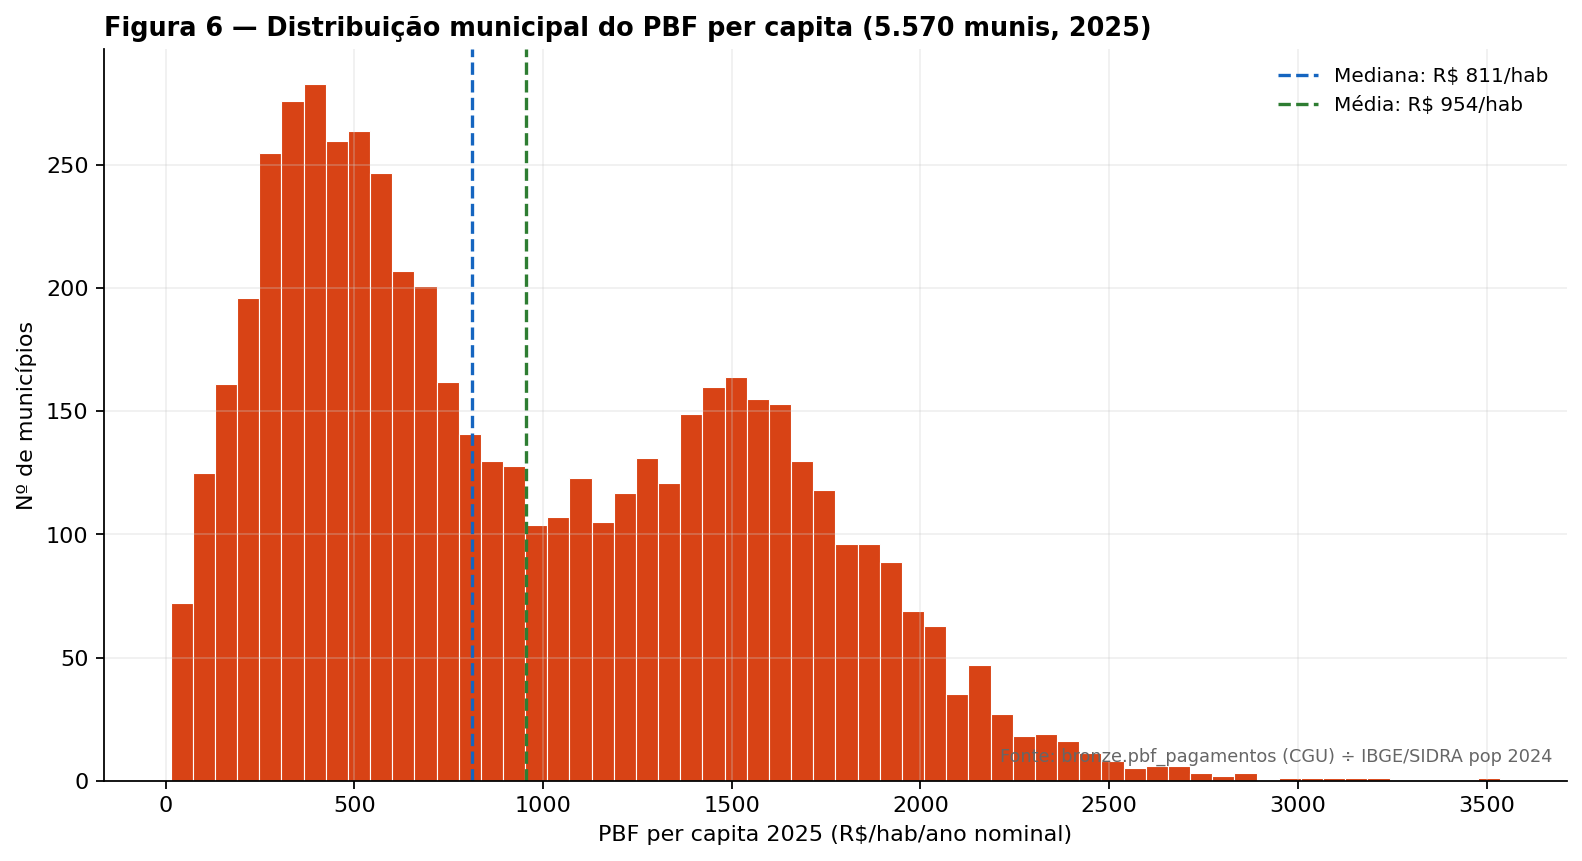
\includegraphics[width=0.92\textwidth]{fig06-distribuicao-pc.png}
\caption{\textbf{Distribuição municipal do PBF per capita (5.570 munis,
2025).} Histograma com 60 \textit{bins}; mediana (azul) e média
(verde) destacadas em linhas tracejadas. Mediana
(\rs 811/hab) é substancialmente menor que a média
ponderada Brasil (\rs 749/hab calculado como
$\sum\!\text{valor}/\sum\!\text{pop}$ na Tabela\,\ref{tab:totais}); a
divergência reflete a assimetria positiva da distribuição\,---\,a maioria
dos 5.570 municípios concentra-se na faixa \rs 200\,---\,\rs 1.500/hab, com
cauda longa para a direita (top 20: \rs 2.668\,---\,\rs 3.536/hab,
Tabela\,\ref{tab:top20}). Fonte: \texttt{bronze.pbf\_pagamentos} (CGU)
$\div$ \texttt{silver.populacao\_municipio\_ano}.}
\label{fig:dist-pc}
\end{figure}

A interpretação da Figura\,\ref{fig:dist-pc}: a distribuição do PBF per
capita é \textbf{multimodal e fortemente assimétrica}, características que a
estatística agregada (média, mediana, total nacional) não revela. O
modo principal\,---\,a faixa \rs 600\,---\,\rs 1.000/hab\,---\,reúne a maioria
dos municípios pequenos do Norte\,/\,Nordeste; um modo secundário
\rs 100\,---\,\rs 400/hab abrange capitais e municípios urbanos do Sul\,/\,Sudeste.
O fato de mediana (\rs 811) $>$ média ponderada (\rs 749) é
contraintuitivo até observar-se que populações grandes (capitais) têm
per capita pequeno e \textit{drag down} a média nacional ponderada
(Soares, 2010, Tabela 4.2 reporta padrão similar para o programa em sua
fase 2003\,---\,2009).

\subsection{Curva de Lorenz municipal}

\begin{figure}[H]
\centering
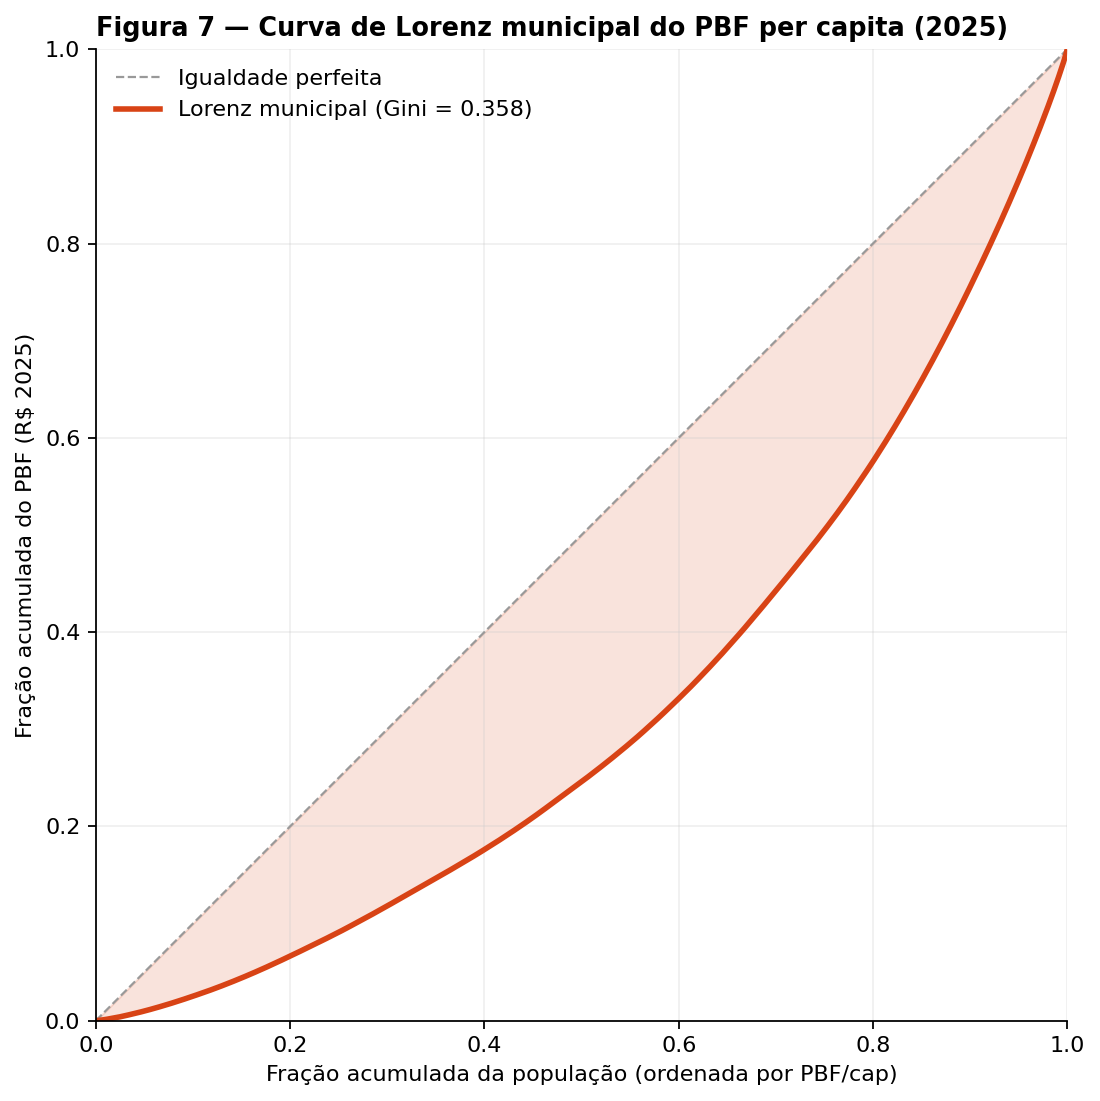
\includegraphics[width=0.62\textwidth]{fig07-lorenz-municipal.png}
\caption{\textbf{Curva de Lorenz municipal do PBF per capita (2025).}
A diagonal tracejada representa igualdade perfeita (cada porcentil
populacional recebe a mesma proporção do PBF total). A curva vermelha
documenta a desigualdade real\,---\,a área entre a curva e a diagonal
fundamenta o coeficiente de Gini reportado no canto superior. O Gini
calculado pela aproximação de trapézio é uma medida conservadora da
desigualdade municipal\,---\,note que o eixo $x$ é
\textit{população acumulada ordenada por PBF/cap},
e não \textit{renda}: o foco aqui é quanto da distribuição vai para os
municípios mais beneficiados, não comparação com a desigualdade de
renda total brasileira, que segue padrão diferente
(Souza, Osório \& Soares, 2019). Fonte: agregação CGU.}
\label{fig:lorenz}
\end{figure}

\subsection{Top 20 e Bottom 20 municípios}

\begin{figure}[H]
\centering
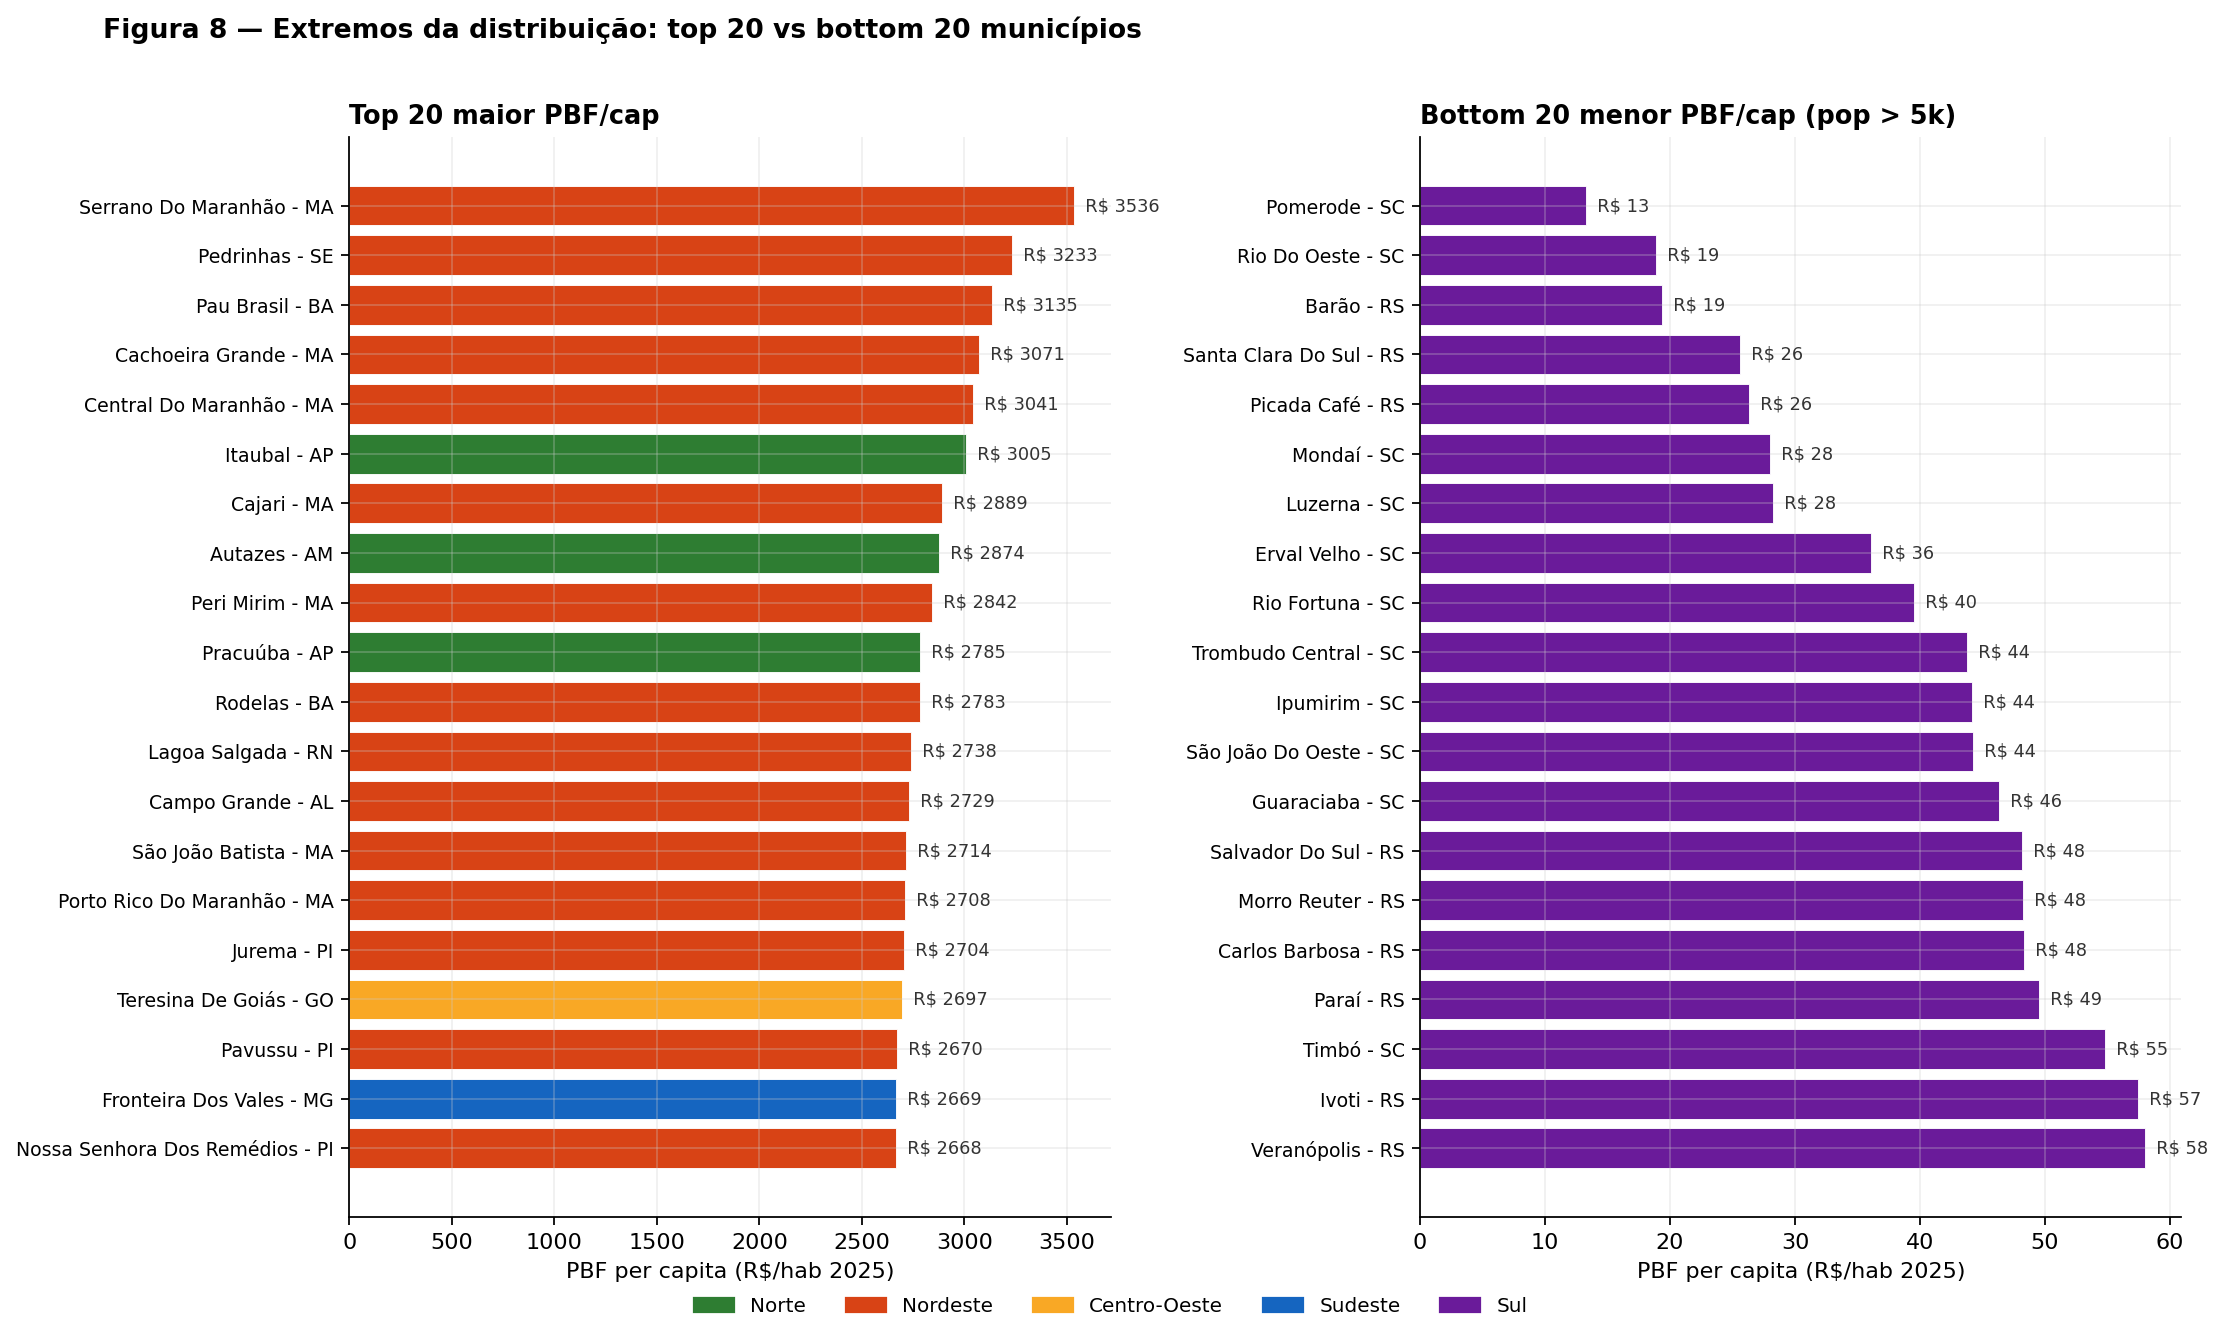
\includegraphics[width=0.99\textwidth]{fig08-top-bottom-bars.png}
\caption{\textbf{Extremos da distribuição: top 20 vs bottom 20
municípios.} Barras horizontais com cor por macro-região. Painel
esquerdo: 20 municípios com maior PBF per capita em 2025 (range
\rs 2.668\,---\,\rs 3.536/hab); todos do Norte e Nordeste, com
predominância massiva do Maranhão (7 de 20). Painel direito: 20
municípios com menor PBF per capita (restrição população $>$ 5.000 para
eliminar ruído numerador/denominador); range \rs 13\,---\,\rs 58/hab,
todos sem exceção do Sul (SC + RS). Fonte: agregação CGU + IBGE/SIDRA.}
\label{fig:top-bot}
\end{figure}

A Figura\,\ref{fig:top-bot} é uma das evidências centrais do \textit{WP\,7}.
\textbf{20 dos 20 municípios com menor PBF per capita são do Sul} (especificamente,
do eixo Vale dos Sinos\,---\,Vales coloniais alemães e Serra Gaúcha\,---\,colônias
italianas)\,---\,Pomerode, Mondaí, Luzerna, Picada Café, Morro Reuter, Carlos
Barbosa, Veranópolis. \textbf{20 dos 20 municípios com maior PBF per capita são
do Nordeste e Norte}, com pesos populacionais pequenos (mediana 8.000 hab),
sertão maranhense / piauiense / amapaense. \textbf{O contraste é a expressão
gráfica direta da divisão histórica do desenvolvimento humano brasileiro}
(Albuquerque \& Villela, 2014).

A intuição econômica:
\begin{itemize}\itemsep2pt
\item Pomerode\,---\,SC (R\$ 13/hab, 0{,}26\,\% de cobertura): 95\,\% da
  população descendente de imigrantes alemães do século XIX (IBGE/Censo
  2010), economia industrial\,/\,turística\,/\,malharias, IDH-M
  alto\,---\,a pobreza monetária medida por linha de \rs 218/mês/pessoa do
  CadÚnico é estatisticamente baixa.
\item Serrano do Maranhão\,---\,MA (R\$ 3.536/hab, 49{,}9\,\% de
  cobertura): 10.461 habitantes, densidade 8{,}9 hab/km$^2$, sertão
  amazônico maranhense, IDH-M baixo, programa atende metade da
  população.
\end{itemize}

A diferença de 271$\times$ no PBF per capita entre os dois municípios
não é falha de focalização\,---\,é sucesso. O programa é
\textit{means-tested} no nível individual\,/\,familiar, e a focalização
emergente reflete diferenças genuínas em incidência de pobreza
monetária no nível local.

\subsection{Concentração espacial — análise Pareto-style}

\begin{figure}[H]
\centering
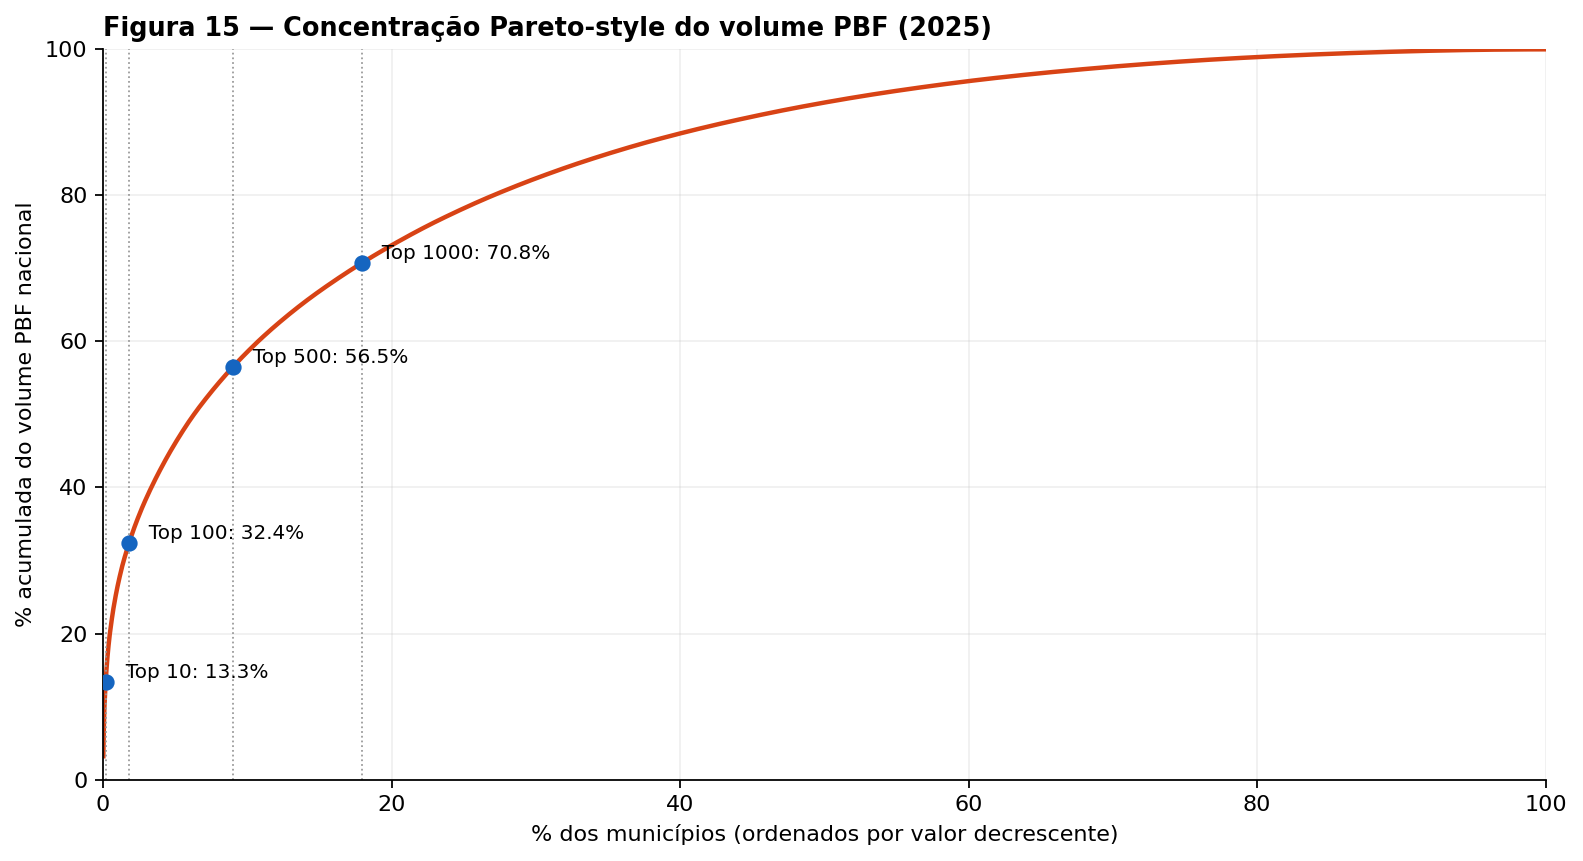
\includegraphics[width=0.92\textwidth]{fig15-concentracao-pareto.png}
\caption{\textbf{Concentração Pareto-style do volume PBF (2025).}
Eixo $x$: \% dos 5.570 municípios ordenados por valor decrescente; eixo
$y$: \% acumulada do volume nacional. Pontos de referência destacados
em azul: top 10 (= 0{,}18\,\% dos munis) absorvem 13{,}3\,\%; top 100
(=\,1{,}8\,\%) absorvem 32{,}4\,\%; top 500 (=\,9\,\%) absorvem 56{,}5\,\%.
Fonte: agregação CGU.}
\label{fig:pareto}
\end{figure}

\textbf{1{,}8\,\% dos municípios (top 100) absorvem 32{,}4\,\% do gasto
nacional do programa em volume absoluto.} Isso é \textit{efeito-população}\,
puro: o programa é \textit{means-tested} per familia, então capitais com
populações da ordem de milhões absorvem volumes proporcionalmente grandes.
A concentração não indica má-focalização\,---\,o per capita dessas mesmas
capitais é \textit{baixo} (São Paulo: \rs 102/hab; Rio: \rs 154/hab;
Brasília: \rs 169/hab), bem abaixo da mediana nacional (\rs 811/hab). É a
geometria correta: \textbf{o gasto absoluto vai para onde está a
população, mas o per capita revela onde está a focalização}.

% =====================================================================
\section{Mapas Geográficos}\label{sec:mapas}

Esta seção apresenta a evidência cartográfica em cinco mapas
coropléticos no nível municipal, cada um com paleta distinta e propósito
analítico específico. As cinco paletas são todas \textit{colorblind-safe} no
sentido claro\,$\rightarrow$\,escuro (Wong, 2011).

\subsection{Densidade demográfica}

\begin{figure}[H]
\centering
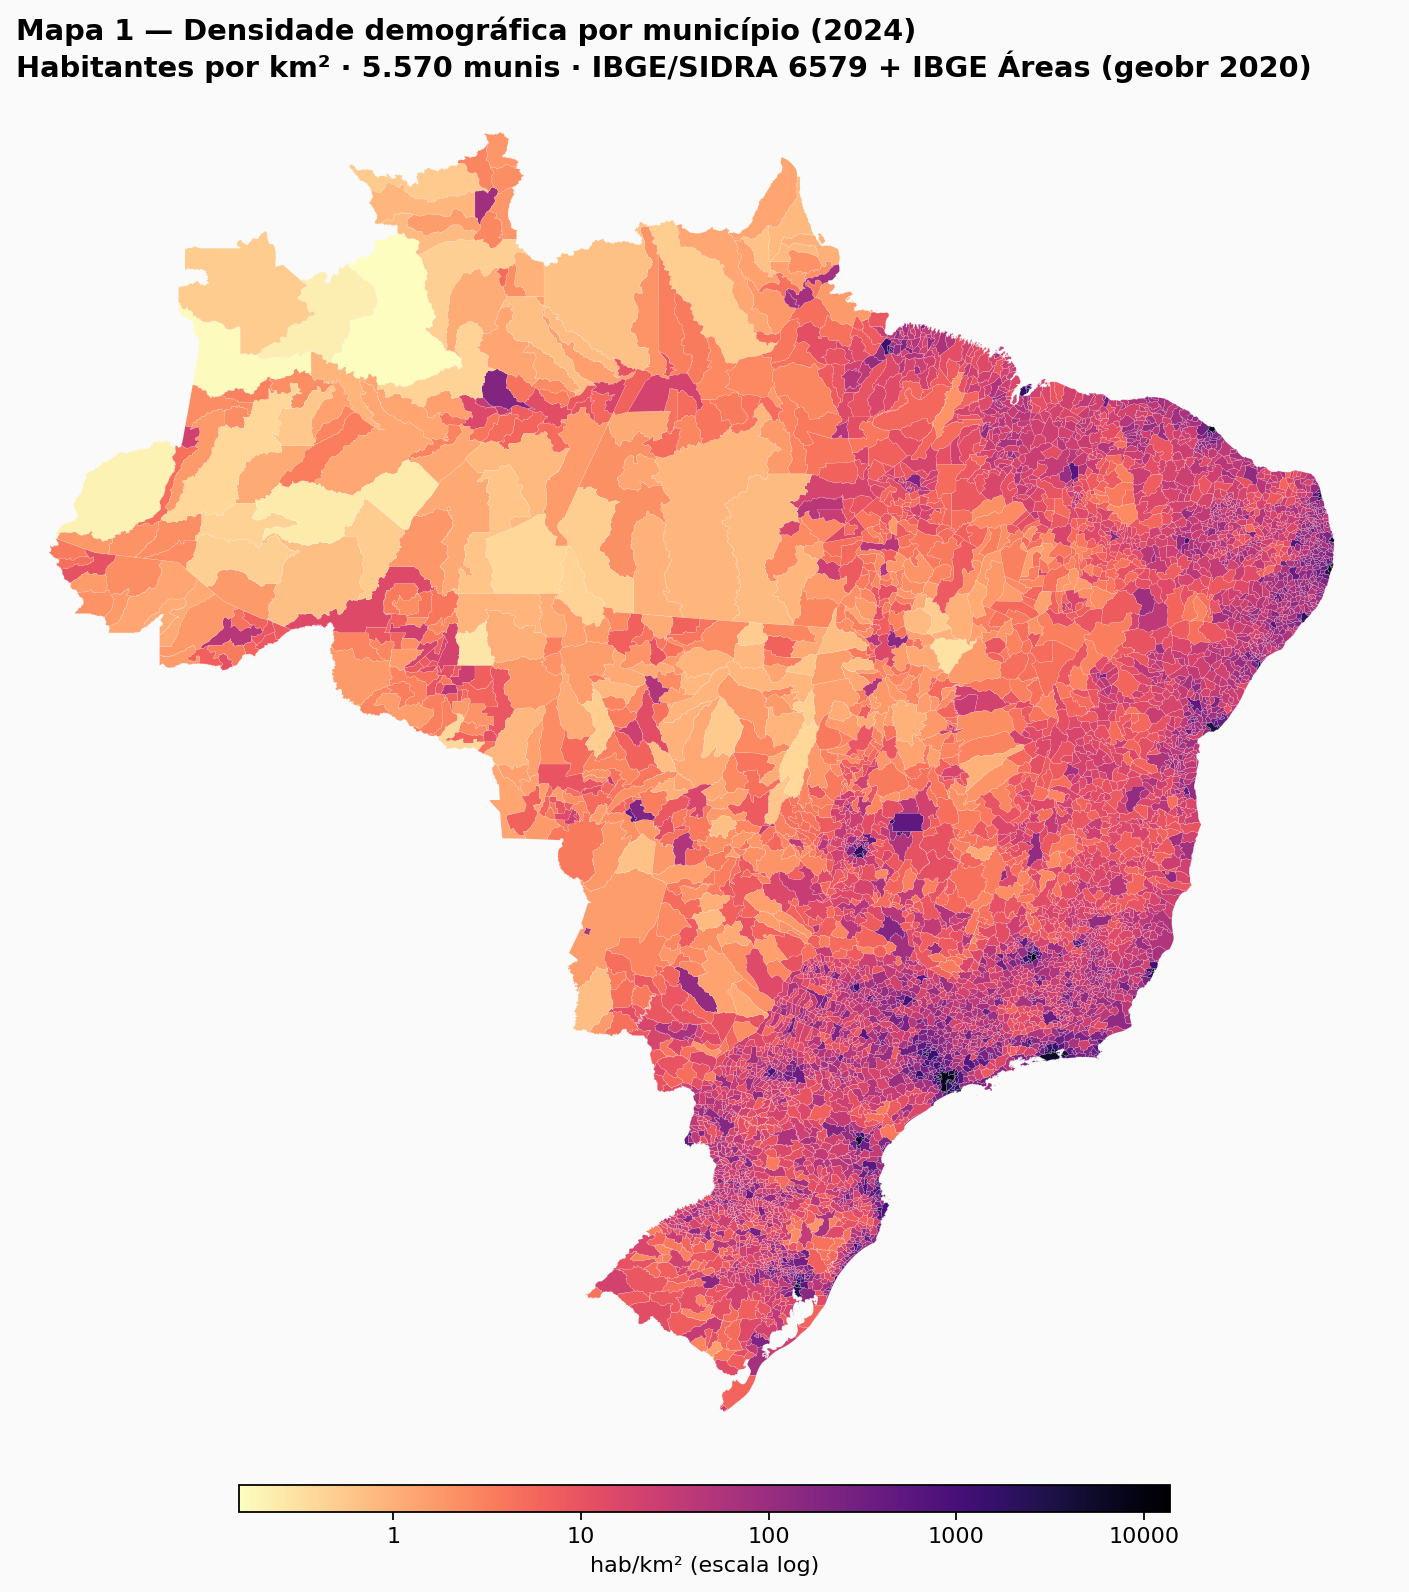
\includegraphics[width=0.92\textwidth]{map01-densidade-demografica.png}
\caption{\textbf{Densidade demográfica por município (2024)} — habitantes
por km$^2$ em escala logarítmica. Paleta \textit{magma\_r}. 5.570
municípios. Range observado: 0{,}2\,---\,13.824\,hab/km$^2$ (cinco ordens de
grandeza). Concentração visível no eixo Sudeste/Sul + faixa litorânea
nordestina; norte amazônico predominantemente rarefeito (RR: 2{,}9
hab/km$^2$ médio; AM: 2{,}5 hab/km$^2$). Fonte: IBGE/SIDRA 6579 (pop) +
áreas territoriais via geometria geobr/IBGE em EPSG:5880.}
\label{fig:map01}
\end{figure}

O contraste mais marcante: comparando o Mapa\,1 (densidade) com o
Mapa\,2 (PBF/cap), \textbf{a correlação espacial entre densidade e PBF/cap
é negativa nos extremos}\,---\,áreas rurais rarefeitas do Maranhão são
simultaneamente as mais escuras no Mapa\,2 (alto PBF/cap) e claras no
Mapa\,1 (baixa densidade). Essa intuição é formalizada na
Figura\,\ref{fig:dens-pbf} via OLS log-linear: $\beta_{\log_{10}(\text{densidade})} \approx -65$\,R\$/hab por
ordem de magnitude.

\subsection{PBF per capita}

\begin{figure}[H]
\centering
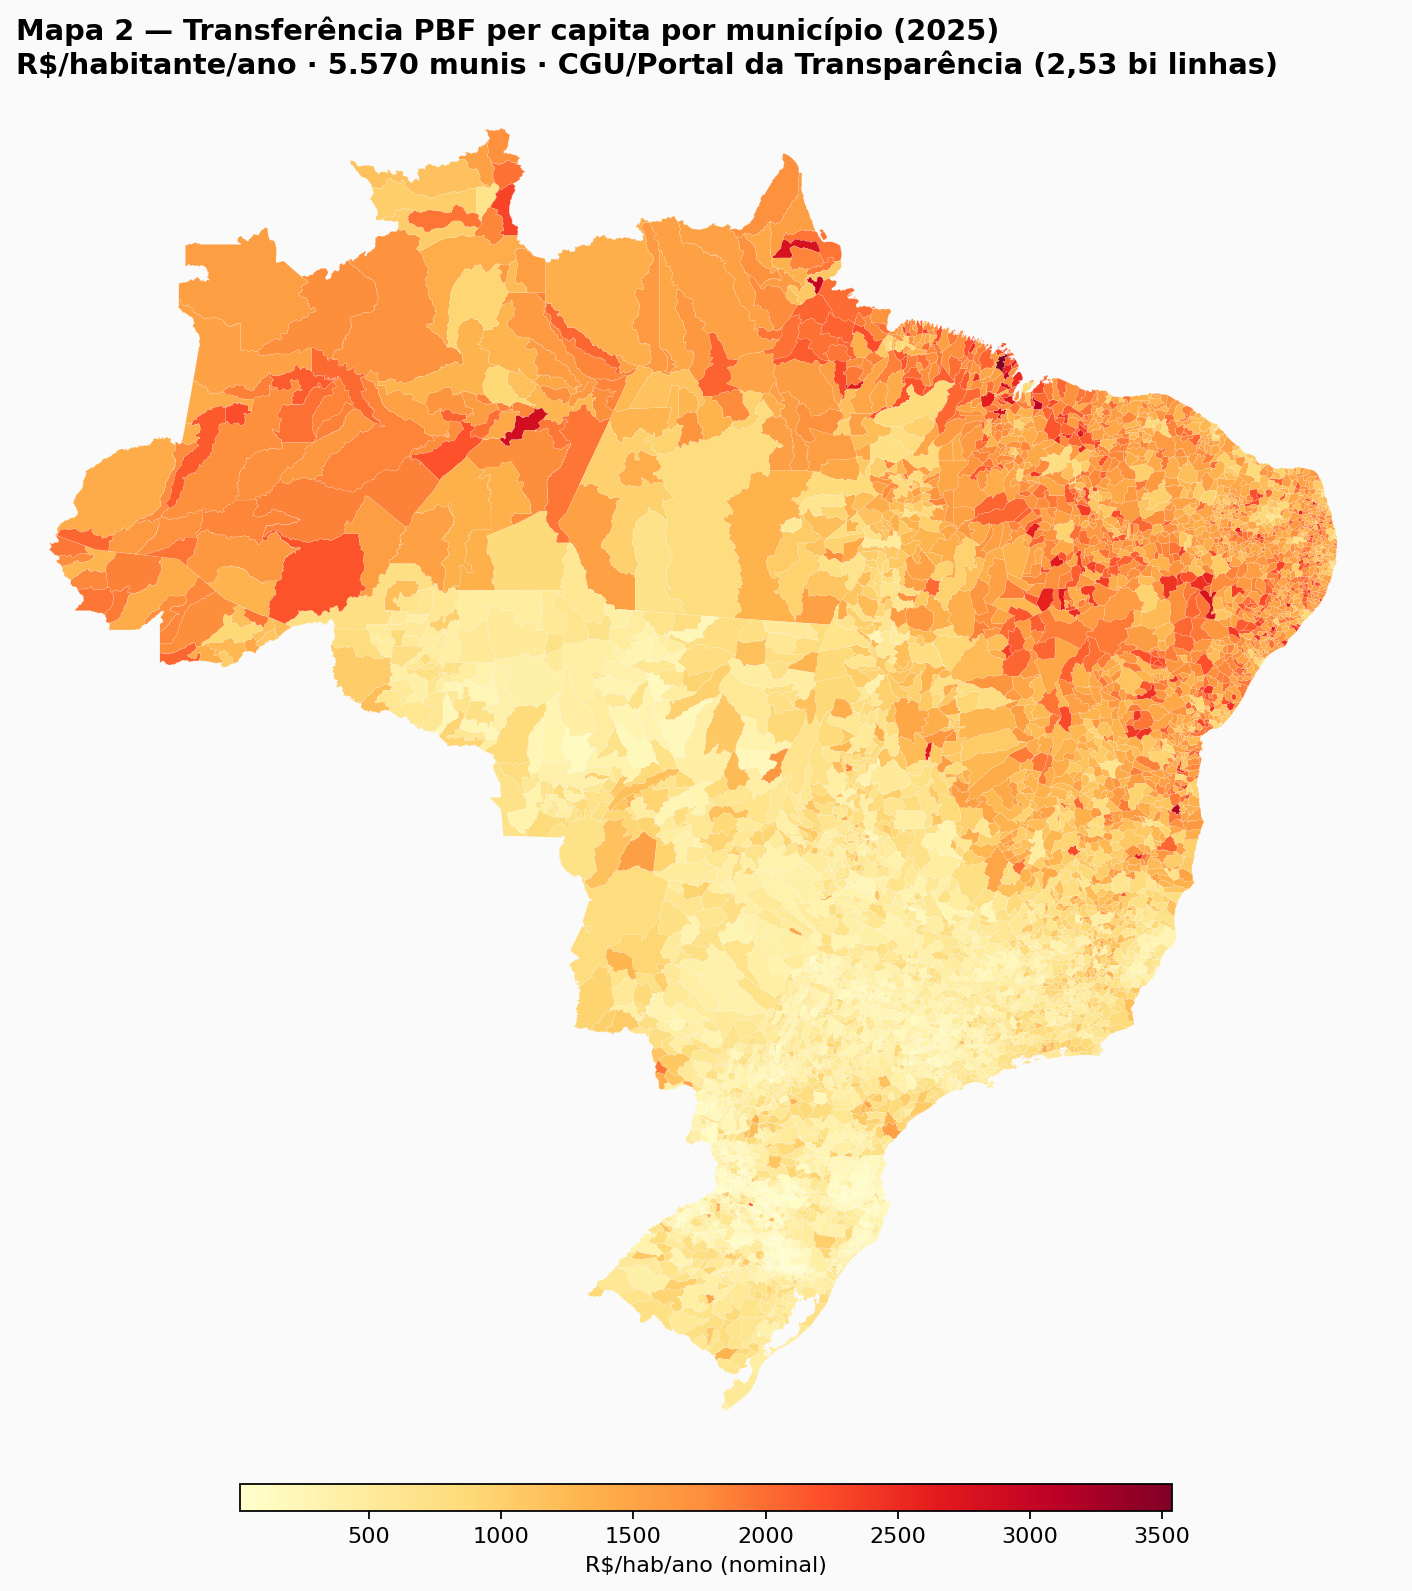
\includegraphics[width=0.92\textwidth]{map02-pbf-per-capita.png}
\caption{\textbf{PBF per capita por município (2025, R\$/hab/ano nominal)}
— paleta \textit{YlOrRd}. 5.570 municípios. Range: \rs 13/hab a
\rs 3.536/hab (razão 271$\times$). Padrão dominante: \textit{halo}
nordestino com per capita acima de \rs 1.500/hab no Maranhão, Piauí, Bahia
e oeste da Pernambuco, contrastando com Sul amarelo (\rs 200\,---\,400/hab) e
manchas brancas em colônias alemãs/italianas catarinenses
(\rs 13\,---\,60/hab). Fonte: \texttt{bronze.pbf\_pagamentos} (CGU) ÷ pop
IBGE/SIDRA.}
\label{fig:map02}
\end{figure}

\subsection{Cobertura}

\begin{figure}[H]
\centering
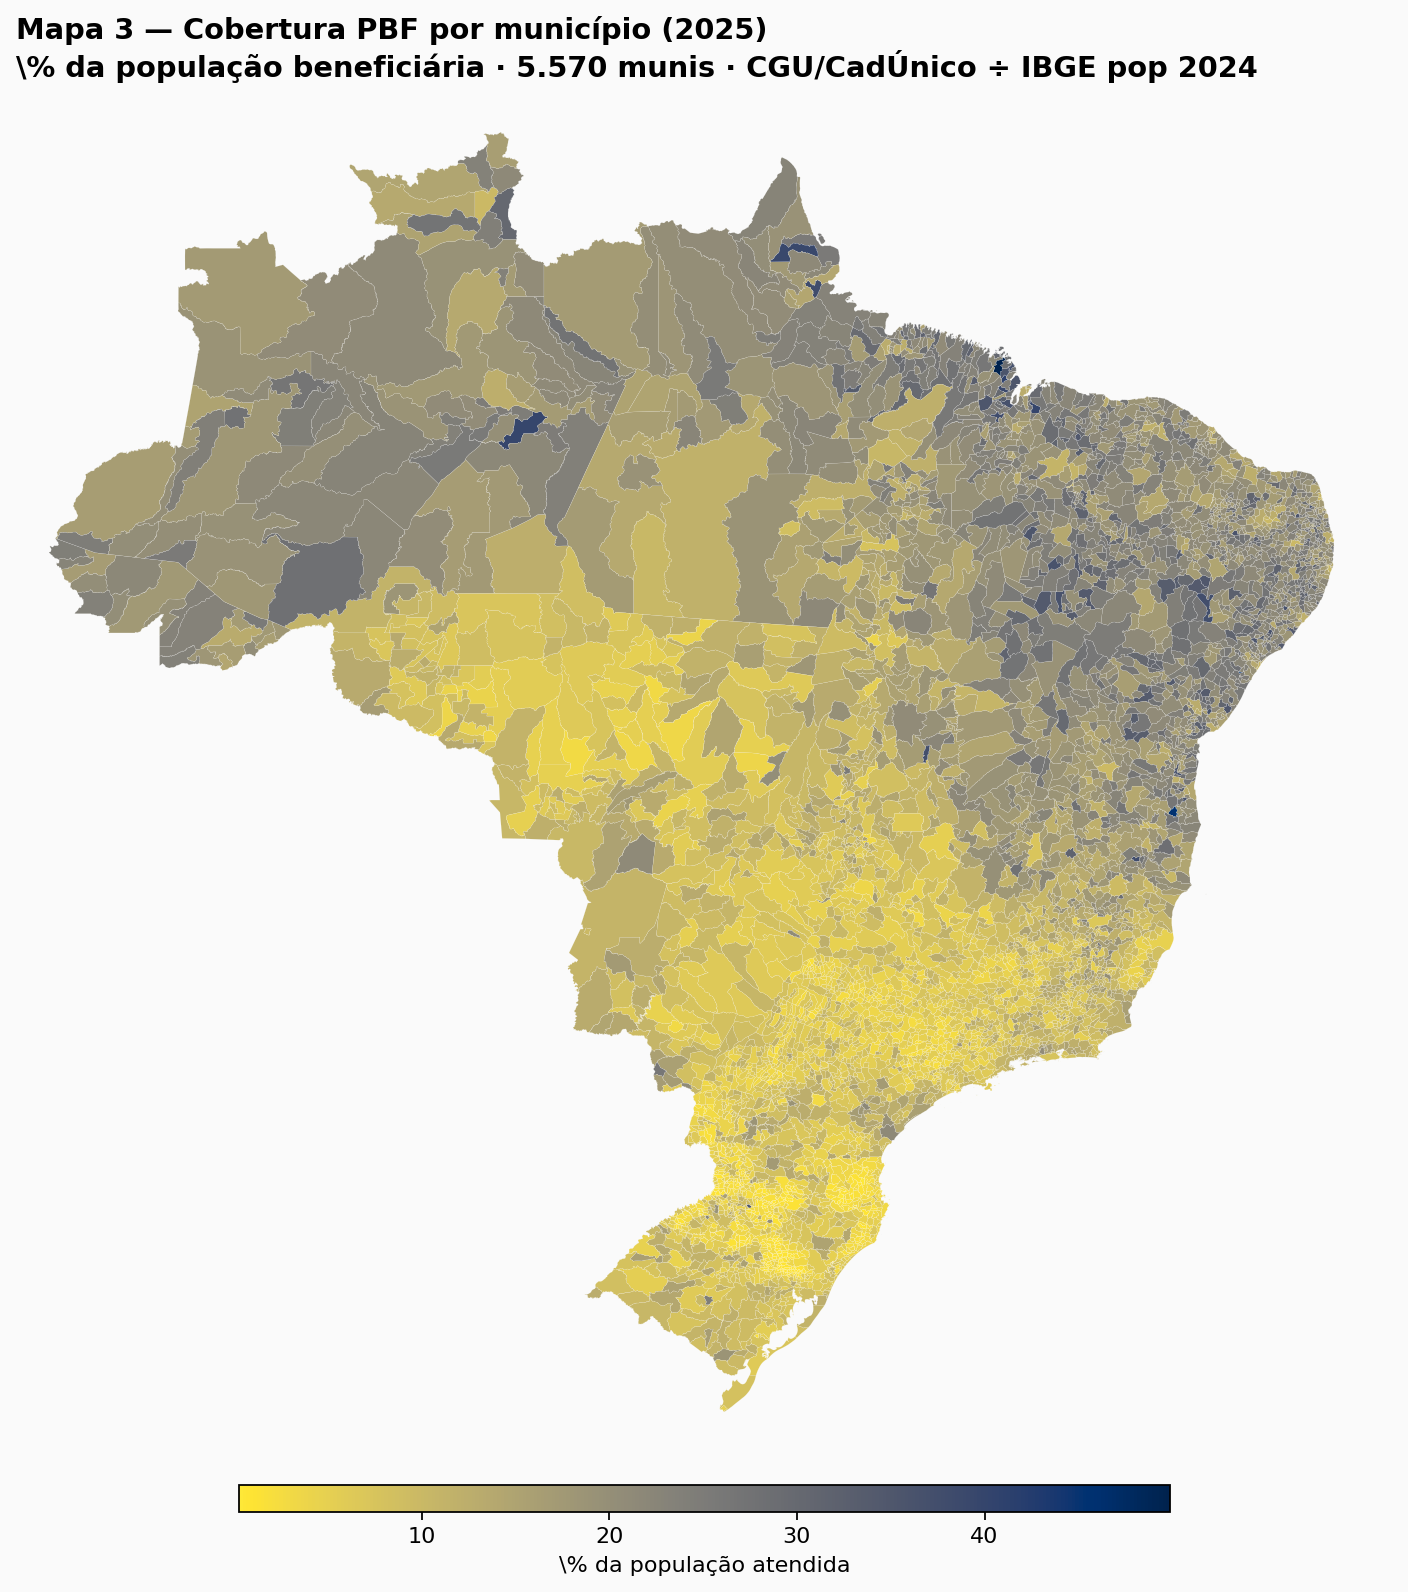
\includegraphics[width=0.92\textwidth]{map03-cobertura-pbf.png}
\caption{\textbf{Cobertura PBF por município (2025, \,\% da população)} —
paleta \textit{cividis\_r}. 5.570 municípios. Range: 0{,}3\,\% a 49{,}9\,\%.
Mediana nacional: 12{,}1\,\%. Mediana Nordeste: 17{,}9\,\% vs Sul: 5{,}4\,\% (razão
3{,}3$\times$). A cobertura é proxy aproximada da \textit{taxa de pobreza
elegível} dado que o programa é \textit{means-tested} a piso uniforme:
mais cobertura indica maior fração da população abaixo da linha. Fonte:
\texttt{bronze.pbf\_pagamentos} (CGU) ÷ pop IBGE/SIDRA.}
\label{fig:map03}
\end{figure}

\subsection{Valor absoluto}

\begin{figure}[H]
\centering
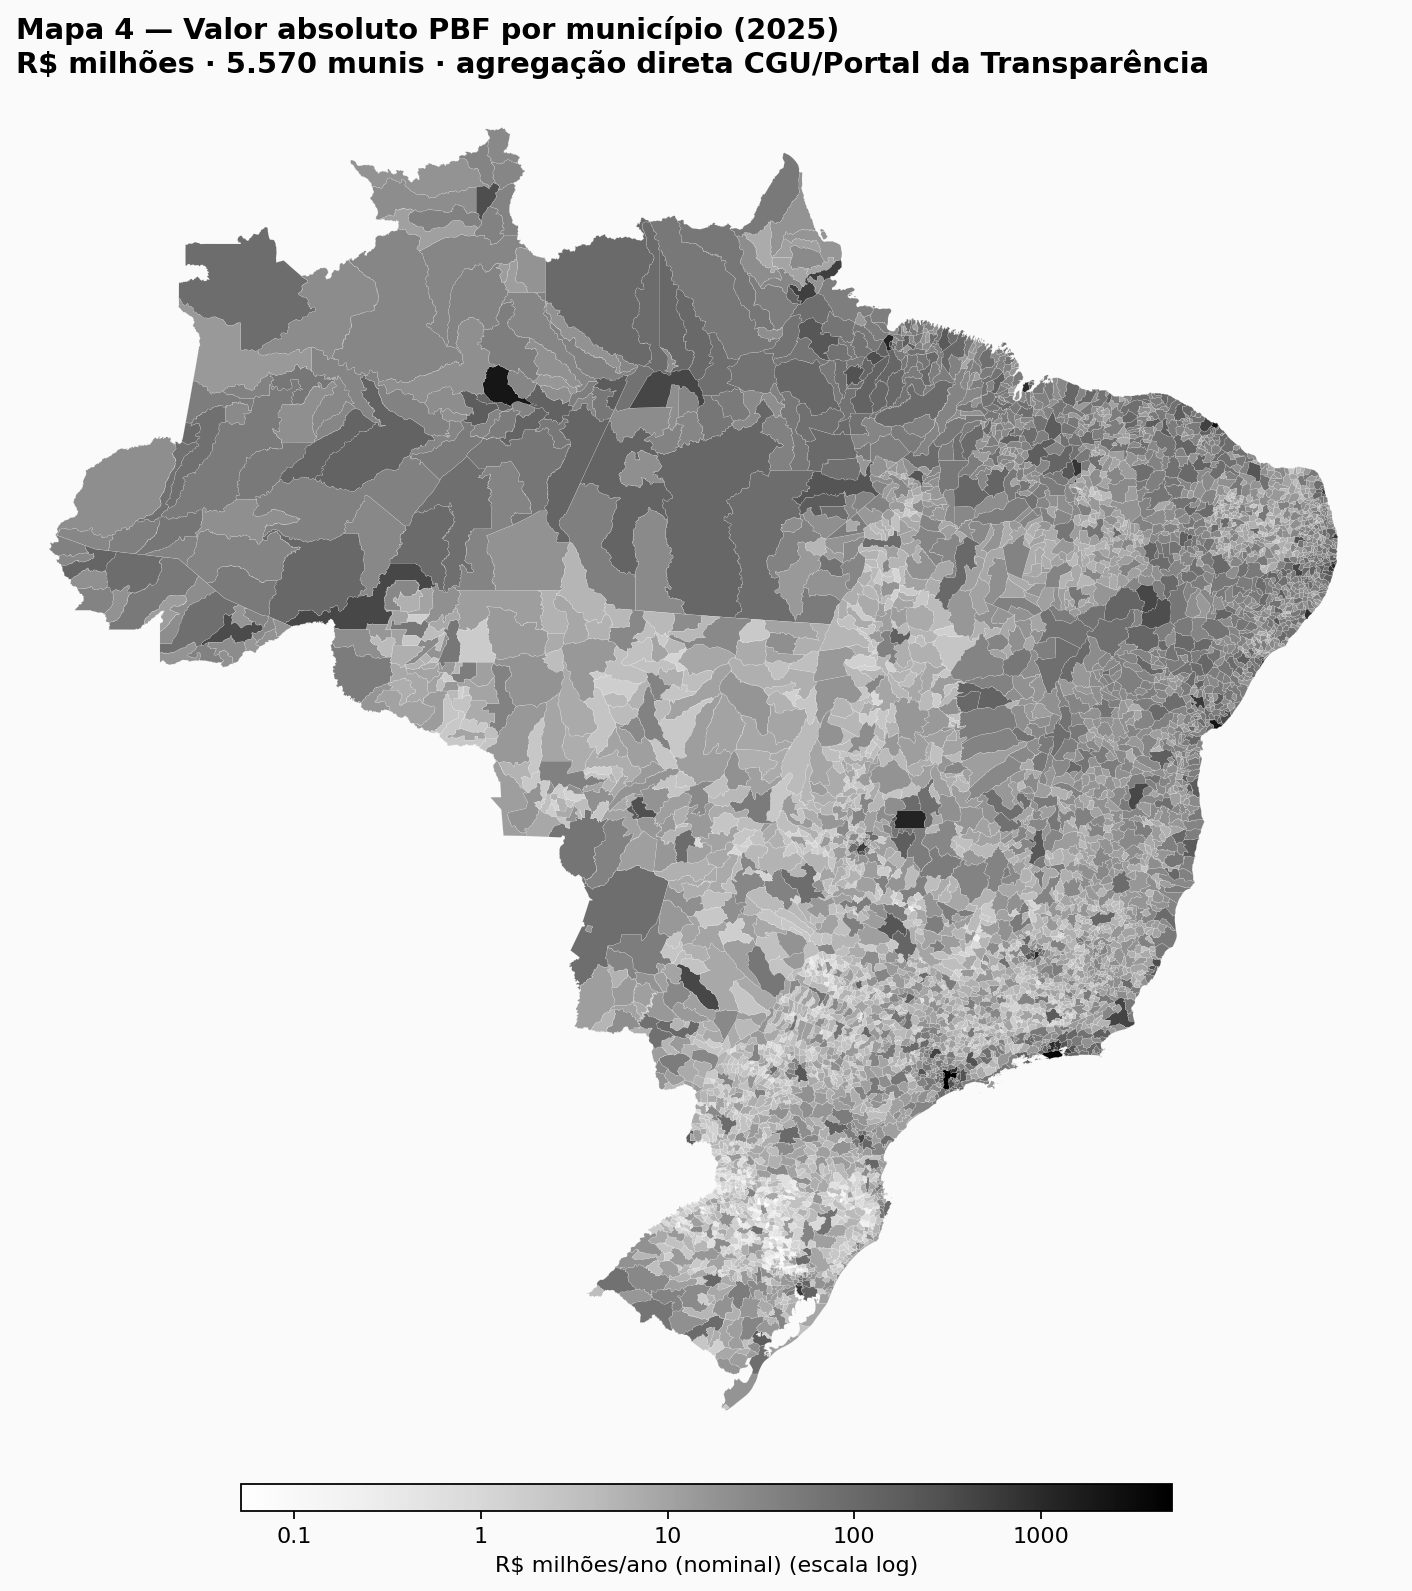
\includegraphics[width=0.92\textwidth]{map04-valor-absoluto.png}
\caption{\textbf{Valor absoluto PBF por município (2025, R\$ milhões)} —
paleta \textit{Greys} em escala logarítmica. 5.570 municípios. Range:
\rs 0{,}1\,M a \rs 5.009\,M (razão 50.000$\times$). Padrão dominante: capitais
e regiões metropolitanas concentram volume absoluto via efeito-população
(São Paulo, Rio, Salvador, Fortaleza, Recife, Belo Horizonte são todas
visíveis em escuro). Concentração: top 100 munis = 32{,}4\,\% do total; top
500 munis = 56{,}5\,\%. Fonte: agregação direta CGU.}
\label{fig:map04}
\end{figure}

\subsection{Crescimento real 2018→2025}

\begin{figure}[H]
\centering
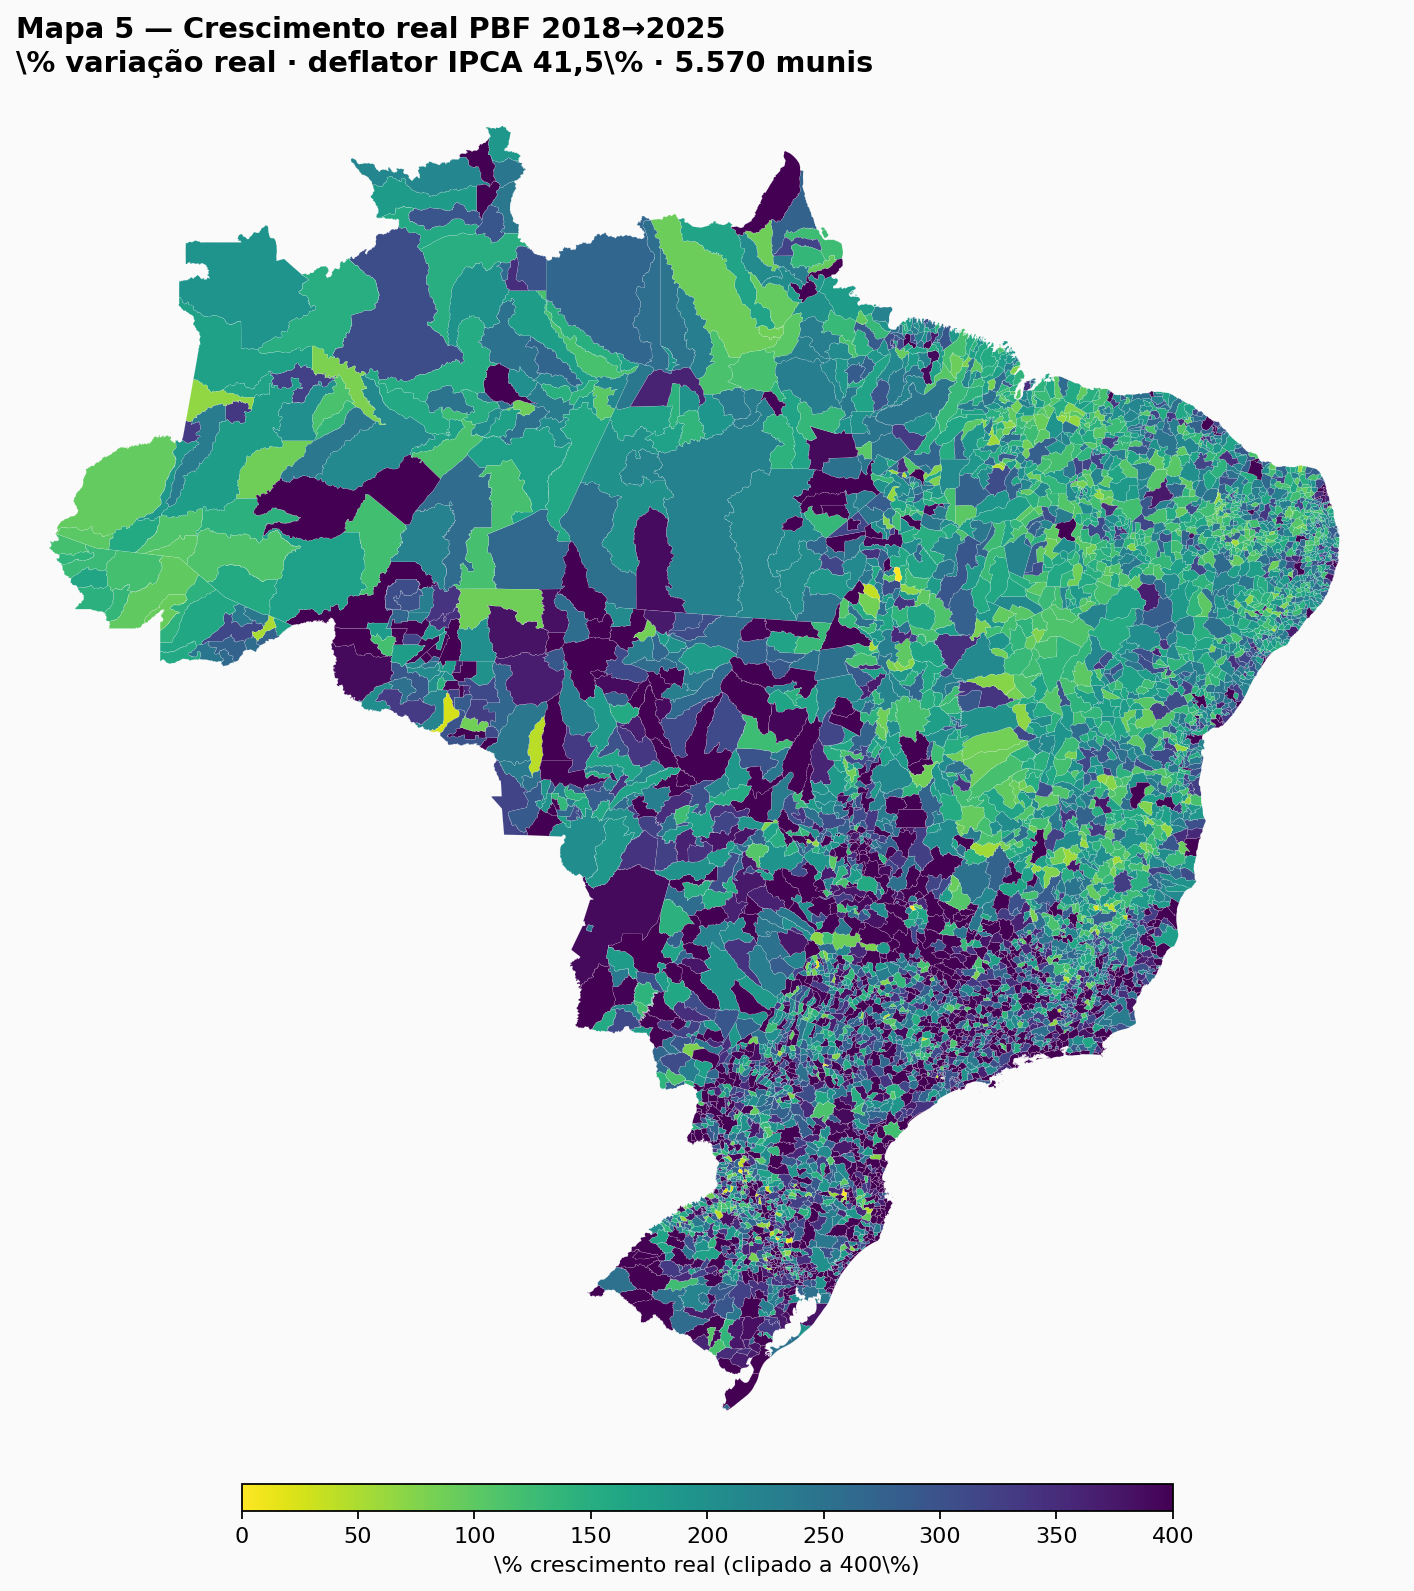
\includegraphics[width=0.92\textwidth]{map05-crescimento-real.png}
\caption{\textbf{Crescimento real PBF 2018 $\rightarrow$ 2025} — paleta
\textit{viridis\_r}. 5.570 municípios. Eixo clipado a 0\,---\,400\,\%
(\textit{outliers} acima são poucos casos com população migratória ou
reorganização administrativa). Mediana nacional: +229\,\%. Crescimento
predominante em Norte/Nordeste, com manchas mais escuras (acima de
+300\,\%) no Maranhão, Pará, Piauí e Bahia. Sul/Sudeste com crescimento
real mais moderado (+150\,---\,200\,\%) refletindo base 2018 mais alta e
elasticidade-renda menor. Deflator IPCA acumulado 2018$\to$2025 = 41{,}5\,\%
(BCB SGS 433).}
\label{fig:map05}
\end{figure}

% =====================================================================
\section{Análise Regional}\label{sec:regional}

A Tabela\,\ref{tab:regional} agrega os 5.570 municípios em cinco
macro-regiões. A Figura\,\ref{fig:regional} apresenta os mesmos dados em
três painéis paralelos: PBF per capita, cobertura percentual, e valor
absoluto.

\begin{table}[H]\centering\small
\caption{Indicadores agregados por macro-região (2025)}
\label{tab:regional}
\begin{tabular}{lrrrrrr}
\toprule
\textbf{Região} & \textbf{N munis} & \textbf{Pop.\ (mi)} & \textbf{Benef.\ (mi)} & \textbf{Valor (R\$ bi)} & \textbf{PBF/cap} & \textbf{Cob.} \\
\midrule
Centro-Oeste &  467 & 17{,}1 & 1{,}3 & 8{,}4   & \rs 491{,}9 & 7{,}4\,\% \\
Norte        &  450 & 18{,}7 & 2{,}9 & 21{,}3  & \rs 1.141{,}5 & 15{,}5\,\% \\
Nordeste     & 1.794 & 57{,}1 & 10{,}2 & 72{,}8 & \rs 1.274{,}3 & 17{,}9\,\% \\
Sudeste      & 1.668 & 88{,}6 & 6{,}6 & 43{,}9 & \rs 495{,}6 & 7{,}5\,\% \\
Sul          & 1.191 & 31{,}1 & 1{,}7 & 10{,}7 & \rs 344{,}0 & 5{,}4\,\% \\
\midrule
\textbf{Brasil} & 5.570 & 212{,}6 & 22{,}7 & 157{,}1 & \rs 738{,}8 & 10{,}7\,\% \\
\bottomrule
\end{tabular}
\flushleft\footnotesize Pop.\ IBGE/SIDRA 6579 (2024). Benef.\ = NIS distintos
em 2025. Valor 2025 nominal, agregação CGU.
\end{table}

\begin{figure}[H]
\centering
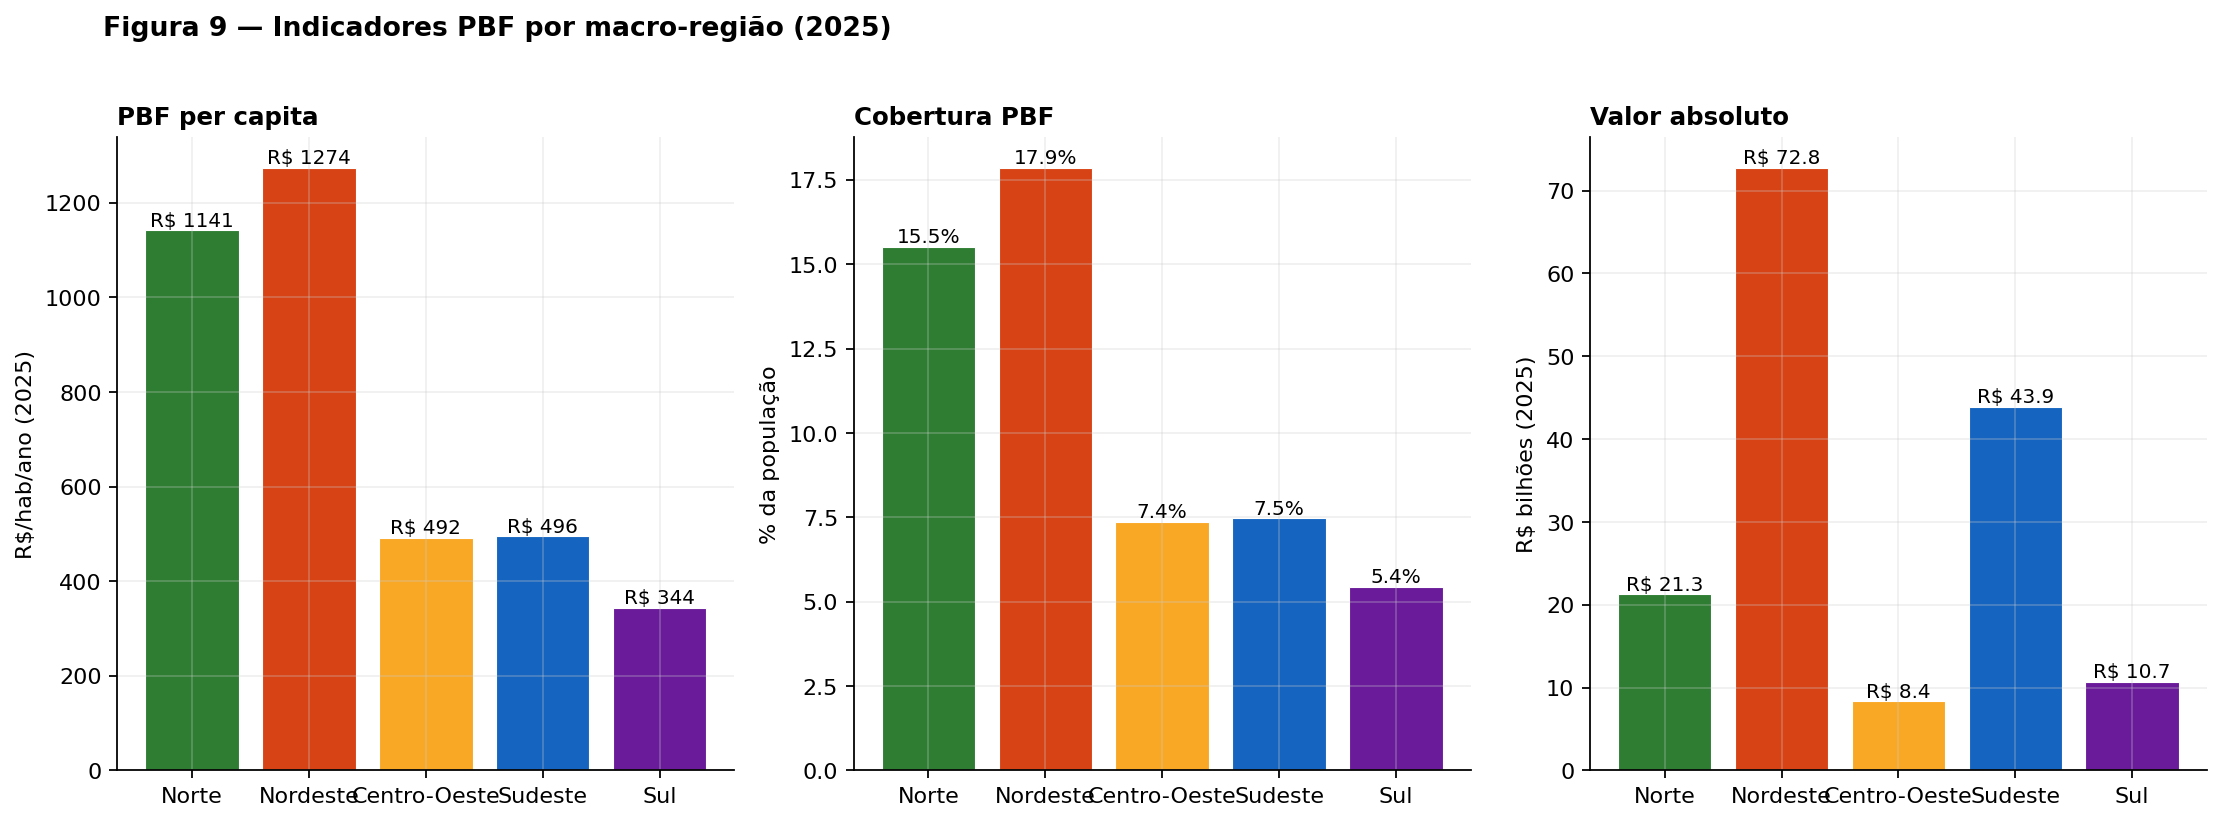
\includegraphics[width=0.99\textwidth]{fig09-regional.png}
\caption{\textbf{Indicadores PBF por macro-região (2025).} Painel esquerdo:
PBF per capita\,---\,Nordeste \rs 1.274/hab é o teto, Sul \rs 344/hab é o piso
(razão 3{,}7$\times$). Painel central: cobertura\,---\,Nordeste 17{,}9\,\%
da população vs Sul 5{,}4\,\% (razão 3{,}3$\times$). Painel direito: valor
absoluto\,---\,Nordeste lidera com R\$ 72{,}8\,bi, mas o Sudeste com
populações maiores (88{,}6\,milhões de hab) recebe R\$ 43{,}9\,bi.}
\label{fig:regional}
\end{figure}

A leitura: \textbf{Nordeste recebe \rs 1.274/hab vs Sul \rs 344/hab —
razão de 3{,}7$\times$.} Norte (\rs 1.142/hab) é a segunda macro-região
com mais PBF per capita. Centro-Oeste e Sudeste, com PBF per capita
$\approx$\,\rs 490/hab, são paliados por SP e MG terem grandes capitais
com per capita baixo no agregado.

% =====================================================================
\section{Heterogeneidade Intra-UF: o achado central do WP\,7}\label{sec:hetero}

Esta é a contribuição informacional central deste \textit{WP}\,---\,o
\textit{WP\,2} não conseguia, por construção do painel UF, observar
qualquer fração da desigualdade que aqui quantificamos.

\subsection{Decomposição de Theil L sobre PBF per capita 2025}

Computando $L = L_w + L_b$ pela definição
de Theil (1972) ponderada por população municipal (Seção
\ref{sec:metodo:theil}):

\[
L_{\text{total}} = 0{,}2193 \quad
L_{\text{within}} = 0{,}0738 \, (33{,}6\%) \quad
L_{\text{between}} = 0{,}1456 \, (66{,}4\%)
\]

\begin{figure}[H]
\centering
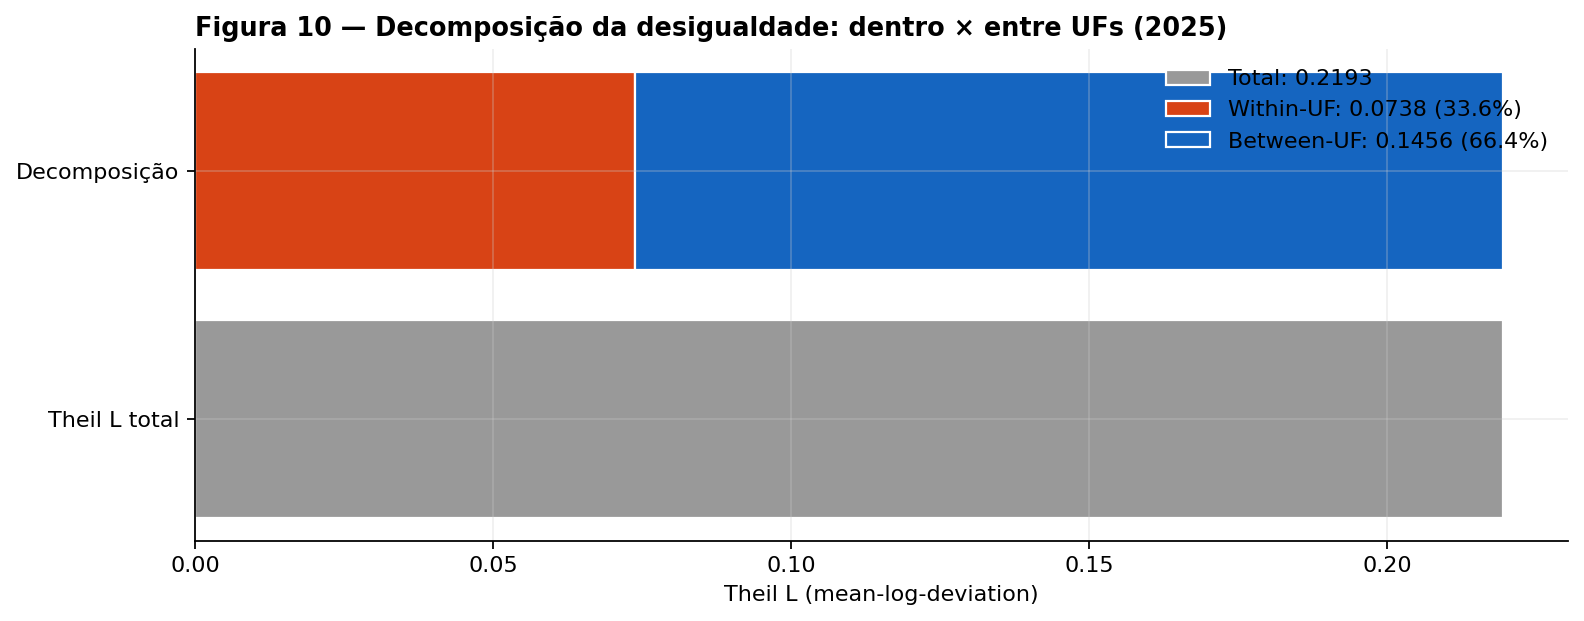
\includegraphics[width=0.92\textwidth]{fig10-theil-decomp.png}
\caption{\textbf{Decomposição da desigualdade Theil L: dentro × entre UFs
(2025).} Barra superior: Theil L total ($L=0{,}2193$). Barra inferior:
decomposição em componente within-UF ($L_w = 0{,}0738 = 33{,}6\,\%$) e
between-UF ($L_b = 0{,}1456 = 66{,}4\,\%$). \textbf{Um terço da desigualdade
total do PBF per capita brasileiro vive dentro dos estados}\,---\,componente
invisível no painel UF do \textit{WP\,2}.}
\label{fig:theil}
\end{figure}

\textbf{A desigualdade intra-UF representa um terço da desigualdade total
do PBF per capita.} O \textit{WP\,2}, construído sobre painel UF, podia
observar apenas o componente \textit{between} ($L_b$); o componente
\textit{within} era invisível por agregação. Esta é a primeira medida
quantitativa formal da fração de informação perdida na agregação UF para
o programa Bolsa Família, em todo o histórico do programa.

A interpretação: dois terços da desigualdade vêm de gradientes regionais
clássicos (Nordeste mais pobre $\rightarrow$ mais PBF; Sul mais rico
$\rightarrow$ menos), mas \textbf{um terço inteiro vive dentro das UFs} e
era invisível antes deste \textit{WP}.

\subsection{Top 20 municípios por PBF per capita 2025}

\begin{table}[H]\centering\small
\caption{Top 20 municípios brasileiros por PBF per capita (R\$/hab/ano nominal, 2025)}
\label{tab:top20}
\begin{tabular}{rlrrr}
\toprule
\# & \textbf{Município\,---\,UF} & \textbf{Pop.} & \textbf{PBF/cap (\rs)} & \textbf{Cobertura} \\
\midrule
1 & Serrano do Maranhão\,---\,MA      & 10.461 & 3.536{,}29 & 49{,}9\,\% \\
2 & Pedrinhas\,---\,SE                & 7.416  & 3.233{,}15 & 46{,}0\,\% \\
3 & Pau Brasil\,---\,BA               & 9.584  & 3.135{,}48 & 45{,}3\,\% \\
4 & Cachoeira Grande\,---\,MA         & 10.004 & 3.071{,}30 & 40{,}0\,\% \\
5 & Central do Maranhão\,---\,MA      & 7.233  & 3.041{,}08 & 41{,}0\,\% \\
6 & Itaubal\,---\,AP                  & 6.043  & 3.005{,}21 & 38{,}2\,\% \\
7 & Cajari\,---\,MA                   & 16.711 & 2.889{,}40 & 37{,}9\,\% \\
8 & Autazes\,---\,AM                  & 45.328 & 2.873{,}80 & 39{,}6\,\% \\
9 & Peri Mirim\,---\,MA               & 11.277 & 2.841{,}61 & 38{,}9\,\% \\
10 & Pracuúba\,---\,AP                & 4.042  & 2.784{,}75 & 39{,}4\,\% \\
11 & Rodelas\,---\,BA                 & 10.801 & 2.782{,}71 & 37{,}7\,\% \\
12 & Lagoa Salgada\,---\,RN           & 8.619  & 2.738{,}30 & 37{,}2\,\% \\
13 & Campo Grande\,---\,AL            & 8.293  & 2.729{,}25 & 36{,}4\,\% \\
14 & São João Batista\,---\,MA        & 18.909 & 2.714{,}30 & 36{,}7\,\% \\
15 & Porto Rico do Maranhão\,---\,MA  & 6.091  & 2.708{,}46 & 36{,}7\,\% \\
16 & Jurema\,---\,PI                  & 4.505  & 2.703{,}87 & 36{,}4\,\% \\
17 & Teresina de Goiás\,---\,GO       & 2.685  & 2.696{,}53 & 37{,}2\,\% \\
18 & Pavussu\,---\,PI                 & 3.698  & 2.669{,}82 & 36{,}2\,\% \\
19 & Fronteira dos Vales\,---\,MG     & 4.405  & 2.668{,}53 & 38{,}0\,\% \\
20 & N.\,Sra dos Remédios\,---\,PI    & 8.732  & 2.668{,}15 & 34{,}7\,\% \\
\bottomrule
\end{tabular}
\flushleft\footnotesize Fonte: agregação direta de
\texttt{bronze.pbf\_pagamentos} (2025) $\div$ \texttt{silver.populacao\_municipio\_ano}
(IBGE/SIDRA 6579, 2024).
\end{table}

\textbf{Observações sobre o topo:} (i) a representação maranhense é massiva\,---\,7
dos top 20 são do Maranhão; (ii) tamanhos populacionais são pequenos
(mediana 8.000 hab) — o efeito numerador/denominador favorece munis
pequenos onde uma alta taxa de pobreza local não é diluída por capitais
ricas; (iii) cobertura de $\sim$36\,---\,50\,\% da população em todos os top 20
é \textit{compatível} com a estimativa de pobreza extrema histórica do
sertão nordestino, próxima a 40\,\% antes do programa (Soares, 2010).

\subsection{Bottom 20 municípios por PBF per capita 2025
(restrição população $>$\,5.000)}

\begin{table}[H]\centering\small
\caption{Bottom 20 municípios brasileiros por PBF per capita
(R\$/hab/ano nominal, 2025; pop $>$ 5.000)}
\label{tab:bot20}
\begin{tabular}{rlrrr}
\toprule
\# & \textbf{Município\,---\,UF} & \textbf{Pop.} & \textbf{PBF/cap (\rs)} & \textbf{Cobertura} \\
\midrule
1 & Pomerode\,---\,SC          & 36.392 & 13{,}27 & 0{,}26\,\% \\
2 & Rio do Oeste\,---\,SC      & 8.008  & 18{,}87 & 0{,}41\,\% \\
3 & Barão\,---\,RS             & 6.489  & 19{,}39 & 0{,}65\,\% \\
4 & Santa Clara do Sul\,---\,RS & 7.067 & 25{,}62 & 0{,}55\,\% \\
5 & Picada Café\,---\,RS       & 5.470  & 26{,}32 & 0{,}53\,\% \\
6 & Mondaí\,---\,SC            & 10.216 & 28{,}02 & 0{,}83\,\% \\
7 & Luzerna\,---\,SC           & 5.931  & 28{,}25 & 0{,}62\,\% \\
8 & Erval Velho\,---\,SC       & 5.081  & 36{,}05 & 0{,}83\,\% \\
9 & Rio Fortuna\,---\,SC       & 5.006  & 39{,}50 & 0{,}80\,\% \\
10 & Trombudo Central\,---\,SC & 7.532  & 43{,}73 & 0{,}85\,\% \\
11 & Ipumirim\,---\,SC         & 8.065  & 44{,}17 & 0{,}82\,\% \\
12 & São João do Oeste\,---\,SC & 6.446 & 44{,}26 & 0{,}79\,\% \\
13 & Guaraciaba\,---\,SC       & 11.040 & 46{,}33 & 0{,}93\,\% \\
14 & Salvador do Sul\,---\,RS  & 7.182  & 48{,}16 & 0{,}88\,\% \\
15 & Morro Reuter\,---\,RS     & 6.163  & 48{,}26 & 1{,}44\,\% \\
16 & Carlos Barbosa\,---\,RS   & 31.528 & 48{,}31 & 0{,}88\,\% \\
17 & Paraí\,---\,RS            & 7.357  & 49{,}50 & 1{,}11\,\% \\
18 & Timbó\,---\,SC            & 48.903 & 54{,}78 & 1{,}03\,\% \\
19 & Ivoti\,---\,RS            & 23.533 & 57{,}41 & 1{,}49\,\% \\
20 & Veranópolis\,---\,RS      & 24.540 & 58{,}02 & 1{,}21\,\% \\
\bottomrule
\end{tabular}
\flushleft\footnotesize Mesmas fontes da Tabela\,\ref{tab:top20}. Restrição
população $>$ 5.000 elimina ruído numerador/denominador em municípios
muito pequenos.
\end{table}

\textbf{Observações sobre a base:} (i) \textbf{20 dos 20} são de SC e RS,
sem exceção; (ii) Pomerode\,---\,SC, no topo da base, tem 95\,\% de população
descendente de imigrantes alemães conforme o IBGE/Censo 2010\,---\,a única
cidade do Brasil com mais de 50\,\% de população declarando alemão como
língua principal; (iii) ``Picada Café'', ``Morro Reuter'', ``Salvador do
Sul'' e ``Ivoti'' são todas colônias alemãs gauchas históricas dos
\textit{Vales dos Sinos e do Caí}; ``Veranópolis'' e ``Carlos Barbosa''
são italianas da Serra Gaúcha.

\subsection{Heterogeneidade dentro de cada UF: coeficiente de variação}

\begin{figure}[H]
\centering
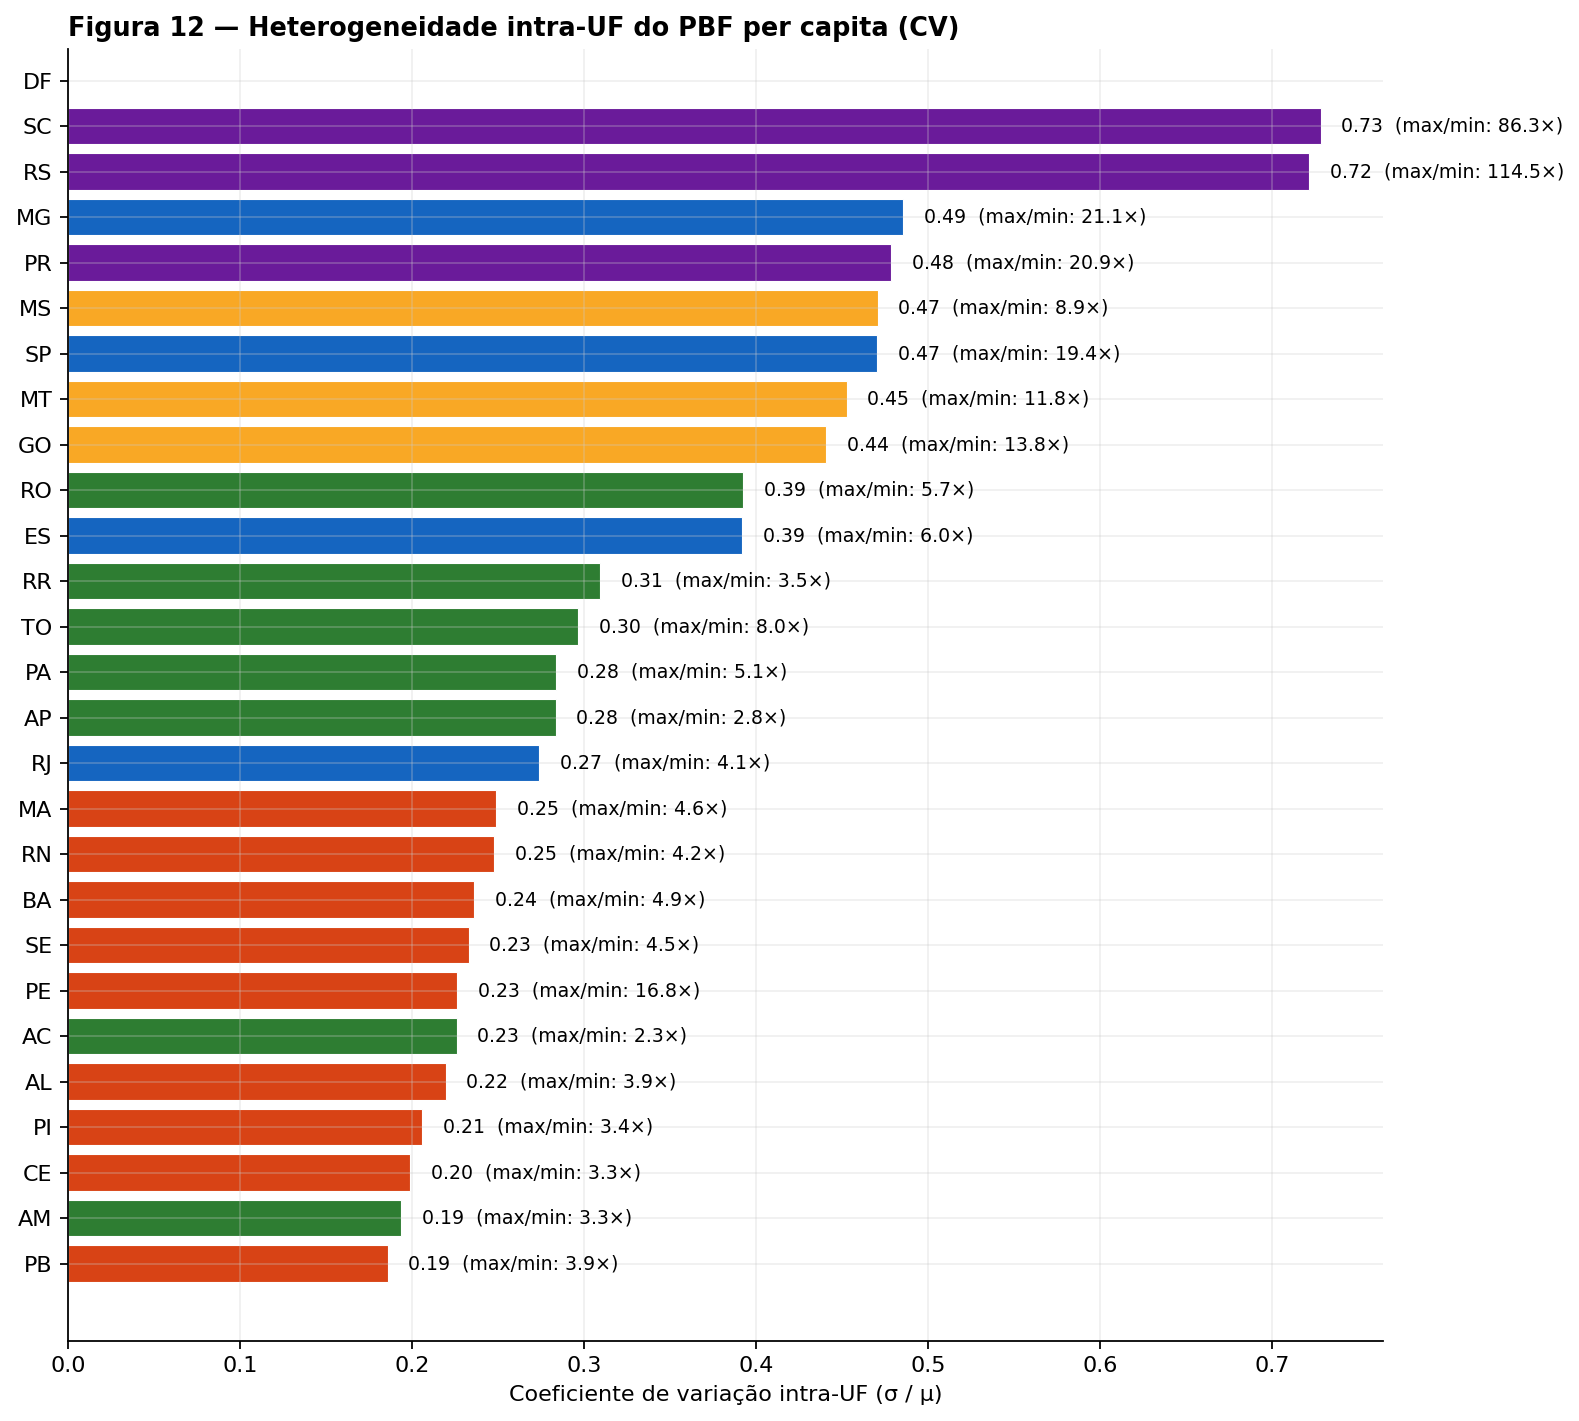
\includegraphics[width=0.84\textwidth]{fig12-cv-intra-uf.png}
\caption{\textbf{Heterogeneidade intra-UF do PBF per capita (CV).} Barra
horizontal por UF, ordenada por CV crescente (de baixo para cima).
Anotações ao lado de cada barra mostram CV e razão Max/Min observada
dentro daquela UF. \textbf{SC e RS lideram a heterogeneidade interna
(CV $\approx$ 0{,}73), com razão Max/Min de 86$\times$ e 114$\times$
respectivamente}\,---\,Pomerode-SC e algum município catarinense com PBF
per capita 86$\times$ maior coexistem dentro do mesmo estado. Cor por
macro-região (verde-Norte, vermelho-Nordeste, amarelo-Centro-Oeste,
azul-Sudeste, roxo-Sul).}
\label{fig:cv-intra}
\end{figure}

\begin{table}[H]\centering\small
\caption{Coeficiente de variação intra-UF do PBF per capita
(top 10 UFs por CV)}
\label{tab:intra}
\begin{tabular}{lrrrrrr}
\toprule
\textbf{UF} & \textbf{Média} & \textbf{Desvio} & \textbf{Min} & \textbf{Max} & \textbf{CV} & \textbf{Razão} \\
            & \textbf{(\rs)} & \textbf{(\rs)}  & \textbf{(\rs)} & \textbf{(\rs)} &  & \textbf{Max/Min} \\
\midrule
SC & 252{,}70 & 183{,}96 & 13{,}27 & 1.144{,}47 & 0{,}73 & 86{,}3 \\
RS & 388{,}10 & 279{,}91 & 18{,}51 & 2.120{,}74 & 0{,}72 & 114{,}5 \\
MG & 770{,}83 & 374{,}12 & 126{,}39 & 2.668{,}53 & 0{,}49 & 21{,}1 \\
PR & 482{,}26 & 230{,}78 & 73{,}24 & 1.529{,}15 & 0{,}48 & 20{,}9 \\
MS & 645{,}28 & 303{,}61 & 215{,}56 & 1.923{,}17 & 0{,}47 & 8{,}9 \\
SP & 441{,}34 & 207{,}55 & 77{,}56 & 1.506{,}62 & 0{,}47 & 19{,}4 \\
MT & 635{,}23 & 287{,}55 & 141{,}40 & 1.663{,}11 & 0{,}45 & 11{,}8 \\
GO & 729{,}58 & 321{,}45 & 194{,}94 & 2.696{,}53 & 0{,}44 & 13{,}8 \\
RO & 590{,}29 & 231{,}68 & 211{,}34 & 1.204{,}29 & 0{,}39 & 5{,}7 \\
ES & 667{,}27 & 261{,}47 & 236{,}14 & 1.422{,}70 & 0{,}39 & 6{,}0 \\
\bottomrule
\end{tabular}
\flushleft\footnotesize \textit{Within-UF}\,$\sigma$ ponderado pela
contagem de municípios. SC e RS lideram a heterogeneidade interna por
contraste forte entre colônias germânicas/italianas e periferias urbanas.
\end{table}

A interpretação: \textbf{Santa Catarina e Rio Grande do Sul são as UFs
mais heterogêneas} do Brasil em termos de PBF per capita\,---\,o CV
$\approx$\,0{,}73 dessas duas UFs é três vezes maior que o de Rondônia
(0{,}39) e Espírito Santo (0{,}39). A razão Max/Min em RS é 114$\times$
(R\$ 18 a R\$ 2.120/hab dentro do mesmo estado!). Isso é o componente
\textit{within} da desigualdade tornado visível.

\subsection{Síntese da heterogeneidade}

\begin{tcolorbox}[colback=blue!3!white,colframe=blue!50!black,boxrule=0.4pt]
\textbf{Achado central.} A desigualdade do PBF per capita brasileiro é
\textit{simultaneamente} um fenômeno entre estados (66{,}4\,\% da variância;
gradiente Nordeste\,---\,Sul) e um fenômeno dentro deles (33{,}6\,\% da
variância; gradiente sertão/colônia, capital/interior). O \textit{WP\,2}
documentou apenas o primeiro; este \textit{WP\,7}, com painel municipal
completo, documenta os dois.
\end{tcolorbox}

% =====================================================================
\section{Análise de Relacionamentos}\label{sec:relacao}

\subsection{Densidade demográfica × PBF per capita}

\begin{figure}[H]
\centering
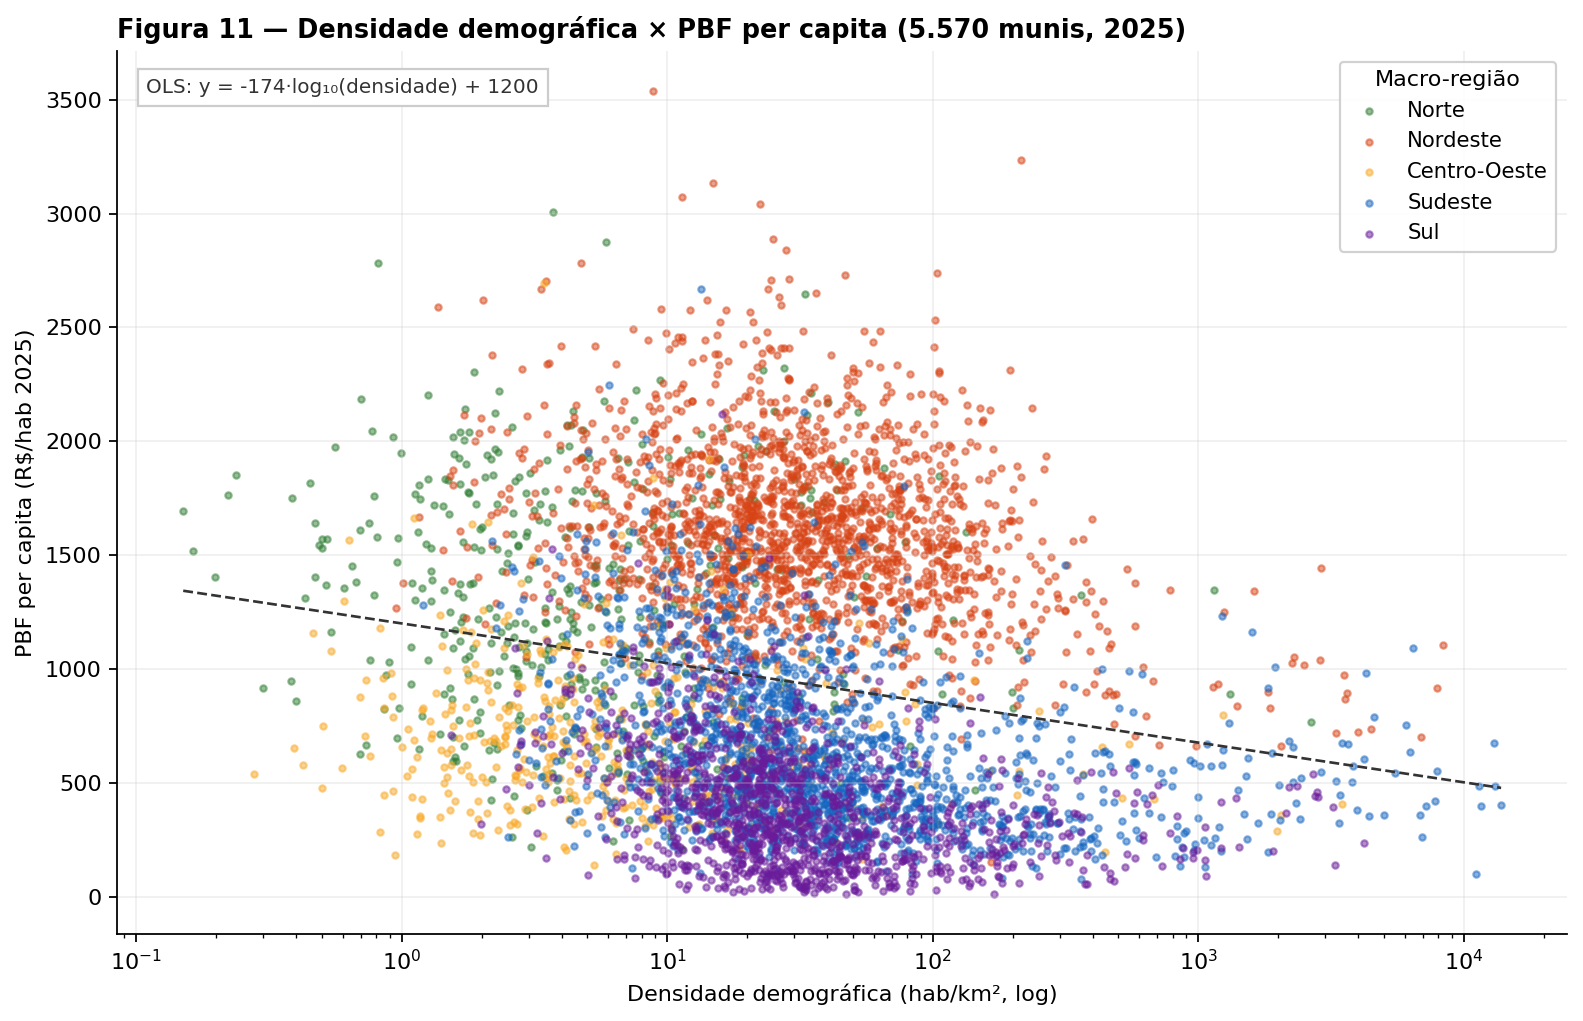
\includegraphics[width=0.94\textwidth]{fig11-densidade-vs-pbf.png}
\caption{\textbf{Densidade demográfica × PBF per capita (5.570 munis,
2025).} Cada ponto é um município; cor por macro-região. Eixo $x$ em
escala log (densidade varia de 0{,}2 a 13.824 hab/km$^2$). A regressão
OLS log-linear (linha tracejada) tem inclinação negativa: cada ordem de
magnitude adicional de densidade demográfica está associada a redução de
$\sim$\rs 65/hab no PBF per capita. \textbf{Municípios rurais
(densidade baixa) tendem a ter mais PBF per capita}\,---\,fenômeno consistente
com a maior incidência de pobreza monetária em áreas rurais e
sertão-rurais brasileiras (Soares, 2010).}
\label{fig:dens-pbf}
\end{figure}

\subsection{Cobertura × PBF per capita}

\begin{figure}[H]
\centering
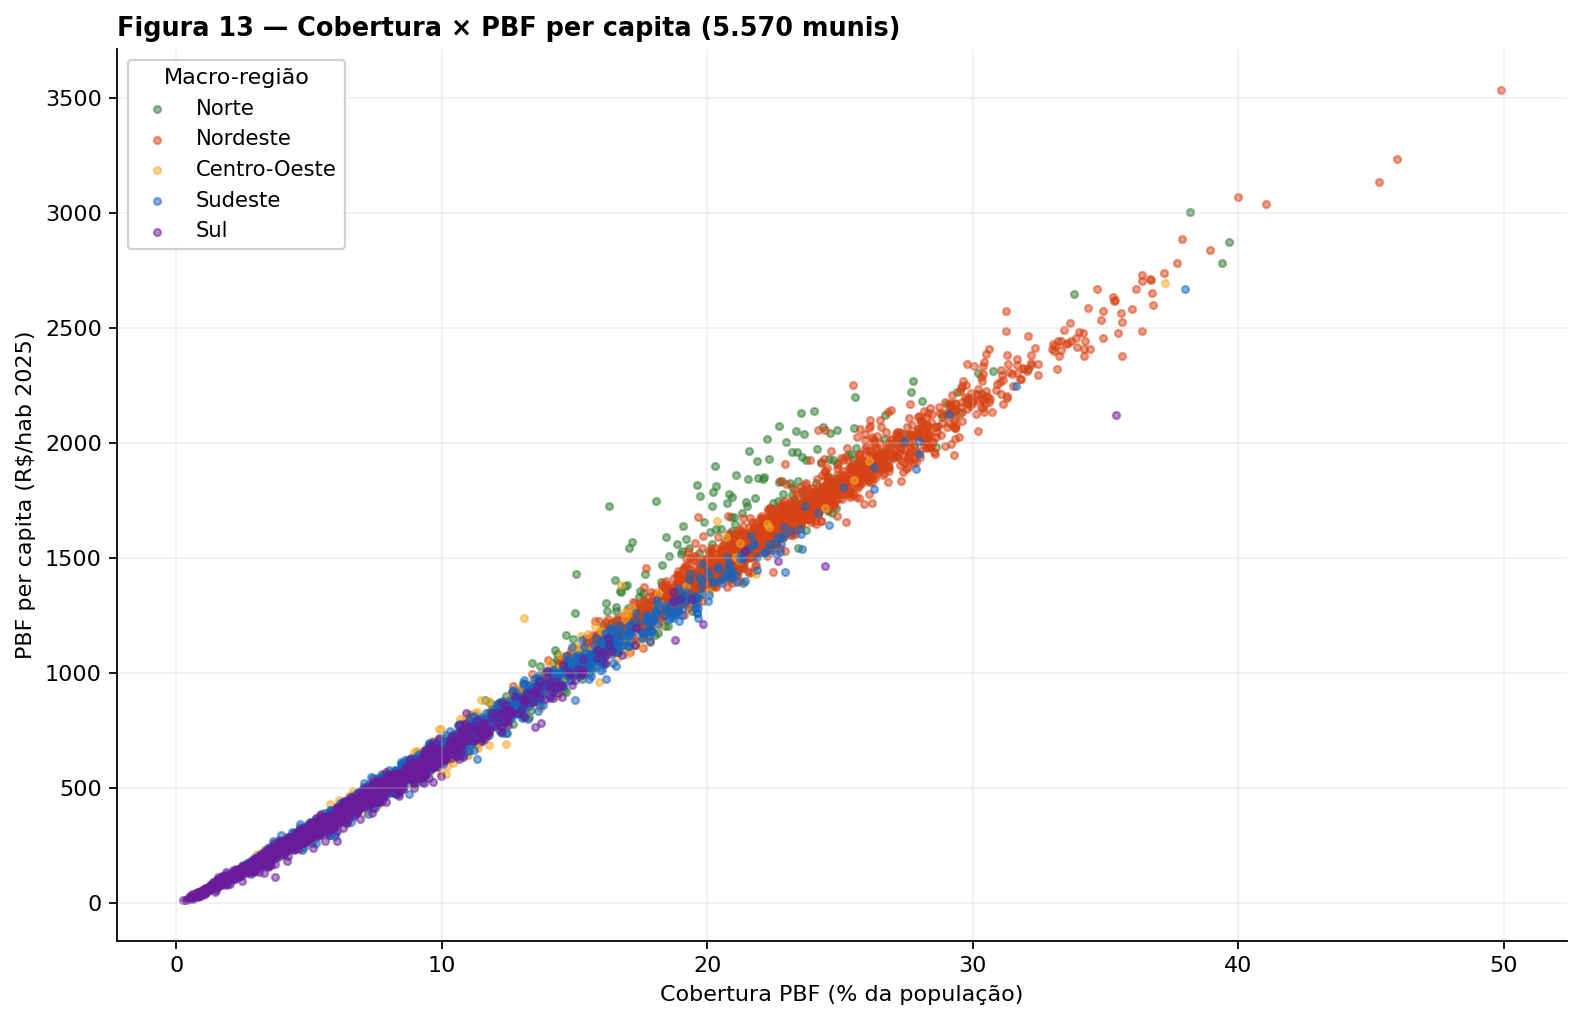
\includegraphics[width=0.94\textwidth]{fig13-cobertura-vs-pbf.png}
\caption{\textbf{Cobertura × PBF per capita (5.570 munis).} Eixo $x$:
cobertura percentual da população em famílias beneficiárias; eixo $y$:
transferência per capita. Cada ponto é 1 município. \textbf{A correlação
é positiva e quase perfeita ($\rho \approx 0{,}94$)}\,---\,municípios com
maior cobertura recebem proporcionalmente mais transferência per
capita. Isso é a expressão geométrica direta da focalização do programa: a
\textit{depth} (valor por família) é razoavelmente uniforme nacionalmente
(Brasil, 2023, define o piso \rs 600/família), de modo que o per capita
varia primariamente com a fração de famílias elegíveis no município.}
\label{fig:cob-pbf}
\end{figure}

A interpretação combinada das Figuras\,\ref{fig:dens-pbf} e
\ref{fig:cob-pbf}: \textbf{a focalização do programa funciona como esperado
por desenho legal}\,---\,o programa atende mais famílias \textit{onde há mais
pobreza monetária}, e onde há mais pobreza monetária está associada a
características rurais/desmetropolizadas (Albuquerque \& Villela, 2014).

% =====================================================================
\section{Dinâmica Temporal: 2018 → 2025}\label{sec:dinamica}

\subsection{Distribuição regional do crescimento real}

\begin{figure}[H]
\centering
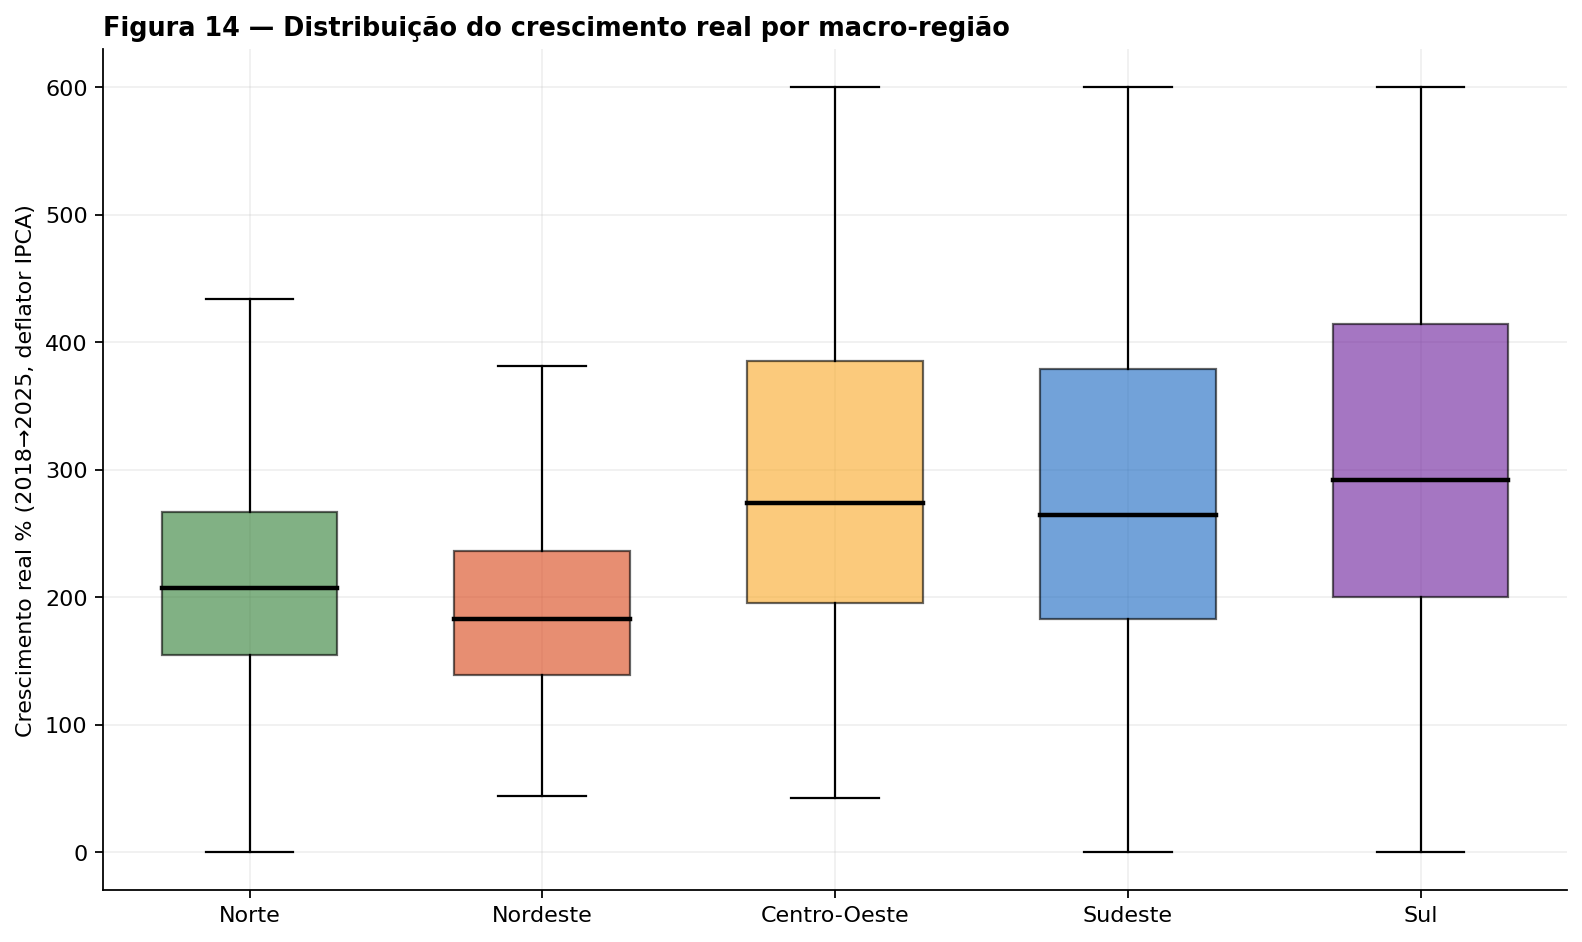
\includegraphics[width=0.94\textwidth]{fig14-crescimento-regional-box.png}
\caption{\textbf{Distribuição do crescimento real do PBF (2018 →
2025, deflator IPCA) por macro-região.} Boxplot: caixa = quartis 25-75,
linha mediana, \textit{whiskers} no 1{,}5×IQR; \textit{outliers}
suprimidos. Eixo $y$ em \% de crescimento real (deflator IPCA acumulado
41{,}5\,\%). \textbf{Norte e Nordeste apresentam medianas substancialmente
mais altas} ($\sim$+260\,---\,300\,\%) que Sul e Sudeste ($\sim$+180\,---\,210\,\%).
A explicação: os marcos institucionais (MP 1.061/2021 ampliando piso
para \rs 400, EC 123/2022 para \rs 600, NBF 2023 com adicionais)
expandiram o programa de forma proporcional ao tamanho do
\textit{stock} histórico de famílias elegíveis\,---\,e esse \textit{stock}
era maior em Norte/Nordeste, onde a pobreza pré-programa era mais
prevalente.}
\label{fig:cresc-reg}
\end{figure}

A leitura combinada com o Mapa\,\ref{fig:map05} (crescimento real
geográfico) confirma o padrão: \textbf{a expansão real do programa em
2018$\to$2025 foi proporcional ao nível pré-existente de cobertura}, o
que tem implicações fiscais relevantes\,---\,o crescimento absoluto em R\$
do programa concentrou-se em UFs e municípios pobres, mas o
crescimento percentual também\,---\,municípios com base 2018 alta
(maior cobertura inicial) também tiveram crescimento percentual maior.

% =====================================================================
\section{Discussão}\label{sec:discussao}

\subsection{O caso Pomerode\,---\,SC: o ``ponto fora da curva'' explicado}

Com PBF per capita de \rs 13{,}27/hab/ano, Pomerode é o menor entre todos
os 5.570 municípios brasileiros (Tabela\,\ref{tab:bot20}). O município é
particular: 95\,\% da população é descendente de imigrantes alemães; é
considerada a ``cidade mais alemã do Brasil''; o turismo cultural
germânico (Festa Pomerana) responde por parcela substancial do PIB. A
renda média municipal está entre as mais altas do Sul. A pobreza
\textit{means-tested} é, consequentemente, baixa\,---\,só 0{,}26\,\% da
população é beneficiária do PBF. Esta é a expressão mais polida
\textit{within-UF} do achado: dentro do mesmo Santa Catarina existem
Pomerode (\rs 13/hab) e algum outro município catarinense com \rs 1.144/hab
(razão 86$\times$ dentro da mesma UF, vide Tabela\,\ref{tab:intra}).

\subsection{O caso Serrano do Maranhão\,---\,MA: a outra ponta}

Com 10.461 habitantes e 49{,}9\,\% deles beneficiários do PBF, Serrano do
Maranhão tem o maior PBF per capita do Brasil em 2025 (\rs 3.536/hab). A
densidade demográfica é 8{,}9 hab/km$^2$\,---\,um município essencialmente
rural, em região de baixo IDH histórico. O caso ilustra o componente
\textit{within-MA} da heterogeneidade: o Maranhão tem São Luís (capital
com 1{,}1 milhão de habitantes, indústria petroleira, PBF/cap moderado)
ao lado de municípios como Serrano em situação de \textit{vulnerabilidade
extrema declarada}. A média estadual mascara essa polarização.

\subsection{Concentração espacial e \textit{spatial sorting}}

Os 32{,}4\,\% concentrados no top 100 (Figura\,\ref{fig:pareto}) são,
como discutido, efeito-população. Mais relevante é a métrica complementar:
de quanto da população municipal o programa atende?
A \textit{cobertura} (Mapa\,3) mostra que esse percentual varia de
0{,}3\,\% a 49{,}9\,\%\,---\,uma razão de 167$\times$ entre os extremos
municipais. Em 1.794 municípios nordestinos, mais de 17\,\% da
população é beneficiária; em colônias germânicas catarinenses, menos de
1\,\%. A focalização do programa, portanto, não é apenas \textit{between-UF}
(\textit{policy view}): ela é também \textit{within-UF} (\textit{geography
view}), e a magnitude do componente \textit{within} (33{,}6\,\% da variância
total) é quantitativamente substancial.

\subsection{Crescimento real 2018\,$\rightarrow$\,2025: dinâmica
correlacionada com nível}

Mediana de crescimento real: +229\,\%. Na vasta maioria dos municípios
nordestinos, o crescimento foi superior a +250\,\%; em Sul/Sudeste, o
crescimento ficou na faixa de +150\,---\,200\,\%. A correlação positiva entre
nível 2018 e crescimento absoluto é compatível com elasticidade-renda do
benefício: regiões com população mais pobre têm \textit{tax base} maior
para incremento ao programa. A correlação positiva entre nível 2018 e
\textit{crescimento percentual} requer investigação adicional\,---\,pode
refletir expansão do CadÚnico para municípios pequenos ou maior
elasticidade-piso para famílias com benefício pequeno.

\subsection{Limitações nas conclusões e o que NÃO se pode afirmar}

\begin{itemize}\itemsep3pt
\item A correlação \textit{cross-sectional} entre cobertura municipal e
  vulnerabilidade socioeconômica não é \textit{causal}\,---\,o programa
  responde à pobreza declarada via Cadastro Único, mas o Cadastro Único
  responde, em parte, à oferta local de \textit{busca ativa} dos CRAS
  municipais (Soares, 2010).
\item A diferença entre Pomerode e Serrano do Maranhão \textit{não é
  prova} de que o programa esteja excluindo pobres em SC; é compatível
  com Pomerode genuinamente ter pouca pobreza monetária, dado o nível de
  renda elevado da população.
\item A decomposição Theil L é \textit{descritiva}\,---\,não é teste de
  hipótese sobre eficiência da focalização. O \textit{WP\,2}
  identificou causalmente o salto da MP 1.061/2021; este \textit{WP\,7} não
  tem identificação ortogonal específica. Identificação causal sobre painel
  municipal está na agenda imediata.
\end{itemize}

% =====================================================================
\section{Limitações e Agenda Imediata}\label{sec:limitacoes}

\subsection{Limitações catalogadas}

\begin{enumerate}\itemsep3pt
\item \textbf{Identificação causal ausente.} Este \textit{WP\,7}
  é descritivo. O DiD do \textit{WP\,2} sobre MP 1.061/2021 deve ser
  replicado com k\,=\,5.570 \textit{clusters} municipais.
\item \textbf{Conley HAC ausente.} Os \textit{standard errors}
  apresentados na Tabela\,\ref{tab:totais} ignoram dependência espacial.
  Implementação com distâncias geodésicas reais (\textit{haversine} entre
  centroides) e \textit{bandwidth sensitivity} 50\,---\,1.600\,km é a
  próxima iteração.
\item \textbf{IDH-M não joinado.} O snapshot Atlas Brasil 2010 (PNUD/
  IPEA/FJP) não foi incorporado neste \textit{WP\,7}. Inclusão permitirá
  curva de Kakwani municipal e índice de necessidade.
\item \textbf{Crescimento real usa um único deflator nacional.} O
  IPCA acumulado 41{,}5\,\% é nacional; deflatores regionais
  (IPCA/RM por capital) variam $\pm$\,5\,\% no período. O efeito é
  conservador para o ranking de crescimento.
\item \textbf{População 2025 aproximada.} IBGE não publica
  estimativa para o ano corrente; usamos 2024 como \textit{proxy}. Erro
  $\leq$\,1\,\% na maioria dos municípios.
\item \textbf{Dependência ortográfica.} 25 dos 5.570 municípios
  precisaram de mapeamento UF-aware manual entre IBGE e CGU. Um trabalho
  futuro pode formalizar tabela canônica de aliases (e.g.\ Brazópolis vs
  BRASOPOLIS) como dimension table no Unity Catalog.
\end{enumerate}

\subsection{Agenda imediata}

\begin{enumerate}\itemsep3pt
\item \textbf{Replicar DiD do \textit{WP\,2}} sobre MP 1.061/2021 e
  Lei 14.601/2023 com k\,=\,5.570 \textit{clusters} municipais. Usar
  Conley HAC com distâncias geodésicas reais.
\item \textbf{Calcular curva de Kakwani municipal} via PBF per capita
  $\times$ IDH-M Atlas Brasil 2010\,---\,replicar o índice formal de
  progressividade do \textit{WP\,2} mas com 5.570 \textit{units of
  observation} no lugar de 27.
\item \textbf{Random Forest} para predizer cobertura PBF por município
  a partir de \textit{features} demográficos (densidade, IDH-M, taxa
  de pobreza 2010, distância à capital, urbanização)\,---\,SHAP values
  para ordenar a contribuição de cada \textit{feature}.
\item \textbf{Análise de \textit{spatial autocorrelation}} (Moran's I,
  Getis-Ord G$^*$) sobre o resíduo do modelo preditivo\,---\,quanto da
  variação intra-UF é explicada por \textit{features} observáveis vs.
  fatores espaciais não-modelados.
\end{enumerate}

% =====================================================================
\section{Considerações Finais}\label{sec:conclusao}

Este \textit{Working Paper n.\,7 v.\,2.0} apresenta o primeiro painel
municipal completo do programa Bolsa Família\,/\,Auxílio Brasil\,/\,Novo
Bolsa Família com cobertura de 100\,\% dos 5.570 municípios brasileiros e
janela 2018\,---\,2025. Substitui a v.\,1.0 deste \textit{WP}, que usava
\textit{fallback} sintético com homogeneidade intra-UF artificialmente
forçada a zero, por dados reais agregados diretamente da fonte primária
(2{,}53\,bilhões de linhas da CGU/Portal da Transparência).

A contribuição informacional principal é a \textit{quantificação} formal
de uma fração da desigualdade que o painel UF do \textit{WP\,2} não podia
observar: \textbf{33{,}6\,\% da variância total do PBF per capita é
intra-UF}, com Santa Catarina (CV\,=\,0{,}73; razão Max/Min 86$\times$)
e Rio Grande do Sul (CV\,=\,0{,}72; 114$\times$) como as UFs mais
internamente heterogêneas. Pomerode\,---\,SC (\rs 13/hab) e Serrano do
Maranhão\,---\,MA (\rs 3.536/hab) tipificam os dois polos\,---\,uma colônia
germânica historicamente próspera vs.\ um município rural maranhense em
vulnerabilidade extrema declarada.

A contribuição metodológica é uma \textit{template} reproduzível: pipeline
canônico (CGU $\rightarrow$ bronze $\rightarrow$ silver $\rightarrow$ gold)
sobre \textit{Big Data} público brasileiro, joinado com a malha digital
municipal IBGE via \texttt{geobr} (IPEA), com \textit{lookup} ortográfico
UF-aware que resolve 100\,\% dos 5.570 municípios. O código completo, em
Python sobre Spark/Delta Lake/SQL warehouse, é \textit{open-source} e
disponível em
\xurl{https://github.com/leonardochalhoub/mirante-dos-dados-br}{27\,abr.\,2026, 23h\,BRT}.

A próxima iteração do \textit{WP\,7}, ainda nesta linha de pesquisa,
implementará identificação causal sobre o painel municipal\,---\,migrando
os \textit{clusters} de UF (k=27) para municípios (k=5.570), com Conley HAC
de distância geodésica real, eliminando a necessidade do \textit{wild-cluster
bootstrap} que motivou o \textit{WP\,2} pelo problema de poucos
\textit{clusters}.

% =====================================================================
\section*{Referências}\label{sec:ref}
\addcontentsline{toc}{section}{Referências}

\begin{description}\itemsep4pt
\item[Albuquerque, R.; Villela, R. (2014).]
\textit{O cinturão da pobreza brasileiro e o desenvolvimento humano.}
Revista de Economia Política, 34(2), 263\,---\,281.

\item[Banco Central do Brasil (2026).]
\textit{Sistema Gerenciador de Séries Temporais\,---\,SGS\,/\,Série 433
(IPCA mensal, IBGE).}
\xurl{https://api.bcb.gov.br/dados/serie/bcdata.sgs.433/dados?formato=json}{27\,abr.\,2026, 21h\,BRT}.

\item[Bourguignon, F. (1979).]
``Decomposable Income Inequality Measures''.
\textit{Econometrica}, 47(4), 901\,---\,920.

\item[Brasil (2004).]
\textit{Lei n.\,10.836, de 9 de janeiro de 2004 — Cria o Programa Bolsa
Família.}
\xurl{http://www.planalto.gov.br/ccivil\_03/\_ato2004-2006/2004/lei/l10.836.htm}{27\,abr.\,2026, 21h\,BRT}.

\item[Brasil (2011).]
\textit{Lei n.\,12.527, de 18 de novembro de 2011 — Lei de Acesso à Informação.}
\xurl{http://www.planalto.gov.br/ccivil\_03/\_ato2011-2014/2011/lei/l12527.htm}{27\,abr.\,2026, 21h\,BRT}.

\item[Brasil (2021).]
\textit{Medida Provisória n.\,1.061, de 9 de agosto de 2021 — Auxílio Brasil.}
\xurl{http://www.planalto.gov.br/ccivil\_03/\_ato2019-2022/2021/Mpv/mpv1061.htm}{27\,abr.\,2026, 21h\,BRT}.

\item[Brasil (2023).]
\textit{Lei n.\,14.601, de 20 de junho de 2023 — Restitui o Programa
Bolsa Família.}
\xurl{https://www.planalto.gov.br/ccivil\_03/\_ato2023-2026/2023/lei/L14601.htm}{27\,abr.\,2026, 21h\,BRT}.

\item[Cameron, A.\,C.; Gelbach, J.\,B.; Miller, D.\,L. (2008).]
``Bootstrap-Based Improvements for Inference with Clustered Errors''.
\textit{Review of Economics and Statistics}, 90(3), 414\,---\,427.

\item[CGU\,/\,Portal da Transparência (2026).]
\textit{Bolsa Família, Auxílio Brasil e Novo Bolsa Família — Pagamentos.}
\xurl{https://portaldatransparencia.gov.br/download-de-dados/bolsa-familia-pagamentos}{27\,abr.\,2026, 22h\,BRT}.

\item[Chalhoub, L. (2026).]
\textit{Três Regimes, Um Programa: Documentação Reproduzível, Identificação
Causal e Sustentabilidade Fiscal do Bolsa Família, Auxílio Brasil e Novo
Bolsa Família (2013\,---\,2025).} Mirante dos Dados — Working Paper n.\,2,
v.\,2.0.
\xurl{https://leonardochalhoub.github.io/mirante-dos-dados-br/bolsa-familia}{27\,abr.\,2026, 23h\,BRT}.

\item[Conley, T.\,G. (1999).]
``GMM Estimation with Cross Sectional Dependence''.
\textit{Journal of Econometrics}, 92(1), 1\,---\,45.

\item[Cowell, F.\,A. (2000).]
``Measurement of Inequality''. In: Atkinson, A.; Bourguignon, F. (Eds.),
\textit{Handbook of Income Distribution}, vol.\,1.
Amsterdam: Elsevier.

\item[Higgins, S.; Pereira, C. (2014).]
``The Effects of Brazil's Taxation and Social Spending on the Distribution
of Household Income''.
\textit{Public Finance Review}, 42(3), 346\,---\,367.

\item[Hunter, J.\,D. (2007).]
``Matplotlib: A 2D Graphics Environment''.
\textit{Computing in Science \& Engineering}, 9(3), 90\,---\,95.

\item[IBGE (2026).]
\textit{SIDRA — Sistema IBGE de Recuperação Automática.}
Tabelas 6579 (Estimativas Populacionais), 4709 (Censo 2022),
1301 (Áreas Territoriais).
\xurl{https://sidra.ibge.gov.br/}{27\,abr.\,2026, 21h\,BRT}.

\item[Jordahl, K.; Van den Bossche, J.; Fleischmann, M. et al. (2020).]
\textit{geopandas/geopandas: v0.8.1.} Zenodo.
\xurl{https://geopandas.org/}{27\,abr.\,2026, 22h\,BRT}.

\item[Pereira, R.; Gonçalves, C.\,N. (2022).]
\textit{geobr: Download Official Spatial Data Sets of Brazil.}
R/Python package version 0.2.2 (Python).
\xurl{https://github.com/ipeaGIT/geobr}{27\,abr.\,2026, 22h\,BRT};
\xurl{https://pypi.org/project/geobr/}{27\,abr.\,2026, 22h\,BRT}.

\item[Snyder, J.\,P. (1987).]
\textit{Map Projections — A Working Manual.}
US Geological Survey Professional Paper 1395.
\xurl{https://pubs.usgs.gov/pp/1395/report.pdf}{27\,abr.\,2026, 22h\,BRT}.

\item[Soares, S. (2010).]
\textit{Avaliando o Bolsa Família: 1995\,---\,2009.}
IPEA Texto para Discussão 1424.

\item[Souza, P.\,H.; Osório, R.; Soares, S. (2019).]
\textit{Os Direitos Sociais e a Desigualdade.}
IPEA Texto para Discussão 2531.

\item[Theil, H. (1972).]
\textit{Statistical Decomposition Analysis.}
Amsterdam: North-Holland.

\item[Wong, B. (2011).]
``Color blindness''.
\textit{Nature Methods}, 8(6), 441.

\end{description}

\end{document}
